%%begin novalidate
\documentclass[12pt]{book}\usepackage[]{graphicx}\usepackage[]{color}
% maxwidth is the original width if it is less than linewidth
% otherwise use linewidth (to make sure the graphics do not exceed the margin)
\makeatletter
\def\maxwidth{ %
  \ifdim\Gin@nat@width>\linewidth
    \linewidth
  \else
    \Gin@nat@width
  \fi
}
\makeatother

\definecolor{fgcolor}{rgb}{0.196, 0.196, 0.196}
\newcommand{\hlnum}[1]{\textcolor[rgb]{0.063,0.58,0.627}{#1}}%
\newcommand{\hlstr}[1]{\textcolor[rgb]{0.063,0.58,0.627}{#1}}%
\newcommand{\hlcom}[1]{\textcolor[rgb]{0.588,0.588,0.588}{#1}}%
\newcommand{\hlopt}[1]{\textcolor[rgb]{0.196,0.196,0.196}{#1}}%
\newcommand{\hlstd}[1]{\textcolor[rgb]{0.196,0.196,0.196}{#1}}%
\newcommand{\hlkwa}[1]{\textcolor[rgb]{0.231,0.416,0.784}{#1}}%
\newcommand{\hlkwb}[1]{\textcolor[rgb]{0.627,0,0.314}{#1}}%
\newcommand{\hlkwc}[1]{\textcolor[rgb]{0,0.631,0.314}{#1}}%
\newcommand{\hlkwd}[1]{\textcolor[rgb]{0.78,0.227,0.412}{#1}}%
\let\hlipl\hlkwb

\usepackage{framed}
\makeatletter
\newenvironment{kframe}{%
 \def\at@end@of@kframe{}%
 \ifinner\ifhmode%
  \def\at@end@of@kframe{\end{minipage}}%
  \begin{minipage}{\columnwidth}%
 \fi\fi%
 \def\FrameCommand##1{\hskip\@totalleftmargin \hskip-\fboxsep
 \colorbox{shadecolor}{##1}\hskip-\fboxsep
     % There is no \\@totalrightmargin, so:
     \hskip-\linewidth \hskip-\@totalleftmargin \hskip\columnwidth}%
 \MakeFramed {\advance\hsize-\width
   \@totalleftmargin\z@ \linewidth\hsize
   \@setminipage}}%
 {\par\unskip\endMakeFramed%
 \at@end@of@kframe}
\makeatother

\definecolor{shadecolor}{rgb}{.97, .97, .97}
\definecolor{messagecolor}{rgb}{0, 0, 0}
\definecolor{warningcolor}{rgb}{1, 0, 1}
\definecolor{errorcolor}{rgb}{1, 0, 0}
\newenvironment{knitrout}{}{} % an empty environment to be redefined in TeX

\usepackage{alltt}

\usepackage[utf8]{inputenc}
\usepackage[T1]{fontenc}
\usepackage[spanish]{babel}
\usepackage{amsmath}
\usepackage{amsthm}
\usepackage{amssymb}
\usepackage{newpxtext,newpxmath}
\usepackage{graphics}
\usepackage{xcolor}
\usepackage{tikz}
\usepackage{mathtools}
\usepackage{graphicx}
\usepackage{hyperref}
\usepackage{setspace}
\doublespacing
\usepackage{csquotes}
\usepackage[style=numeric-comp, sorting=none]{biblatex}
\addbibresource{bibliografia.bib}
%\usepackage{animate}
\usepackage{media9}

%\usepackage[margin=2cm]{geometry}

\usepackage{tcolorbox}
\tcbuselibrary{theorems}
\tcbuselibrary{breakable}

\newtcbtheorem[number within=section]{nota}{Nota}%
{breakable, colback=yellow!5, colframe=yellow!40!gray,
	fonttitle=\bfseries}{nota}

\newtcbtheorem[number within=section,use counter
	from=nota]{cuidado}{Cuidado}%
{breakable, colback=red!5, colframe=red!50!gray,
	fonttitle=\bfseries}{cuidado}

\newtcbtheorem[number within=section,use counter
	from=nota]{tarea}{Tarea}%
{breakable, colback=blue!5, colframe=blue!35!black,
	fonttitle=\bfseries}{tarea}

\newtcbtheorem[number within=section,use counter
	from=nota]{solucion}{Solución}%
{breakable, colback=gray!5, colframe=gray!35!black,
	fonttitle=\bfseries}{sol}

\newtcbtheorem[number within=section,use counter
	from=nota]{pregunta}{Pregunta}%
{breakable,  colback=green!5, colframe=green!35!black,
	fonttitle=\bfseries}{preg}

\newtcbtheorem[number within=section,use counter
	from=nota]{ejemplo}{Ejemplo}%
{breakable, colback=magenta!10, colframe=magenta!50!black,
	fonttitle=\bfseries}{ej}

\newtcbtheorem[number within=section,use counter
	from=nota]{laboratorio}{Laboratorio}%
{breakable, colback=purple!10, colframe=purple!50!black,
	fonttitle=\bfseries}{lab}
%%end novalidate

%%% DEFINICIÓN DE ESTILOS DE TEOREMAS %%%
\theoremstyle{definition}
\newtheorem{definicion}{Definición}

\theoremstyle{plain}
\newtheorem{teorema}{Teorema}
\newtheorem{lema}{Lema}
%%%%%%%%%%%%%%%%%%%%%%%%%%%%%%%%%%%%%%%%%
\IfFileExists{upquote.sty}{\usepackage{upquote}}{}
\begin{document}

%% NO EDITAR %%%%%
%%begin novalidate





%%end novalidate
%%%%%%%%%%%%%%%%

\title{Notas del curso CA-403}
\author{}
\date{}
\maketitle





\section*{Instrucciones de uso}

Este es un archivo de \LaTeX normal, salvo que se le pueden agregar códigos de R.

Para hacerlo solo debe encerrar su código con lo siguiente comandos.

\

\noindent\verb|<<>>=|

\verb|Su código acá.|

\noindent\verb|@|

\

Algunas recomendaciones iniciales:

\begin{itemize}
	\item Tratemos de ser ordenados con el texto y el código. Recuerden que esto será usado por ustedes en el examen.
	\item No usen comandos propios (\texttt{newcommand}) ya que eso solo haría más difícil que los compañeros puedan editar su trabajo.
	\item El documento es colaborativo, por lo que está bien editar o escribir ``encima'' de otro compañero, siempre y cuando esto sea para mejorar el texto.
\end{itemize}

Creo en el buen juicio de cada uno para hacer estas notas lo mejor posible.

\begin{minipage}[c]{0.5\textwidth}
	Para entender mejor la estructura de estas notas, pueden revisar este enlace \url{https://www.overleaf.com/learn/latex/Knitr}
\end{minipage}

\newpage
\include{cap-0-instrucciones.Rtex}








\chapter{Estimación de densidades}

\section{Histograma}

El histograma es una de las estructuras básicas en estadística. Básicamente con este objeto se puede visualizar la distribución de los datos sin tener conocimiento previo de los mismos.

\subsection{Construcción Estadística}

Suponga que  \(X_1,X_2, \dots ,X_n\) proviene de una distribución desconocida.

\begin{itemize}
	\item Seleccione un origen \(x_0\) y divida la linea real en \emph{segmentos}.
	      \begin{equation*}
		      B_j = [x_0 +(j - 1)h,x_0 + jh) \quad j\in \mathbb{Z}
	      \end{equation*}

	\item Cuente cuántas observaciones caen en cada segmento. \(n_j\).

\begin{knitrout}
\definecolor{shadecolor}{rgb}{1, 1, 1}\color{fgcolor}\begin{kframe}


{\ttfamily\noindent\itshape\color{messagecolor}{\#\# `stat\_bin()` using `bins = 30`. Pick better value with `binwidth`.}}\end{kframe}
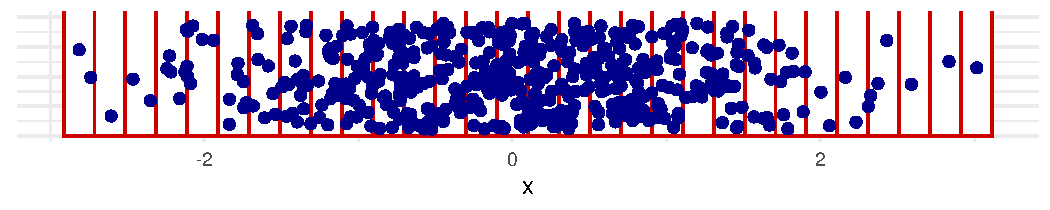
\includegraphics[width=\maxwidth]{figure/observaciones-histograma-1} 

\end{knitrout}

	\item Cuente la frecuencia por el tamaño de muestra \(n\) y el ancho de banda \(h\).
	      \begin{equation*}
		      f_j = \frac{n_j}{nh}
	      \end{equation*}

	\item  Dibuje el histograma.

\begin{knitrout}
\definecolor{shadecolor}{rgb}{1, 1, 1}\color{fgcolor}\begin{kframe}


{\ttfamily\noindent\itshape\color{messagecolor}{\#\# `stat\_bin()` using `bins = 30`. Pick better value with `binwidth`.}}\end{kframe}
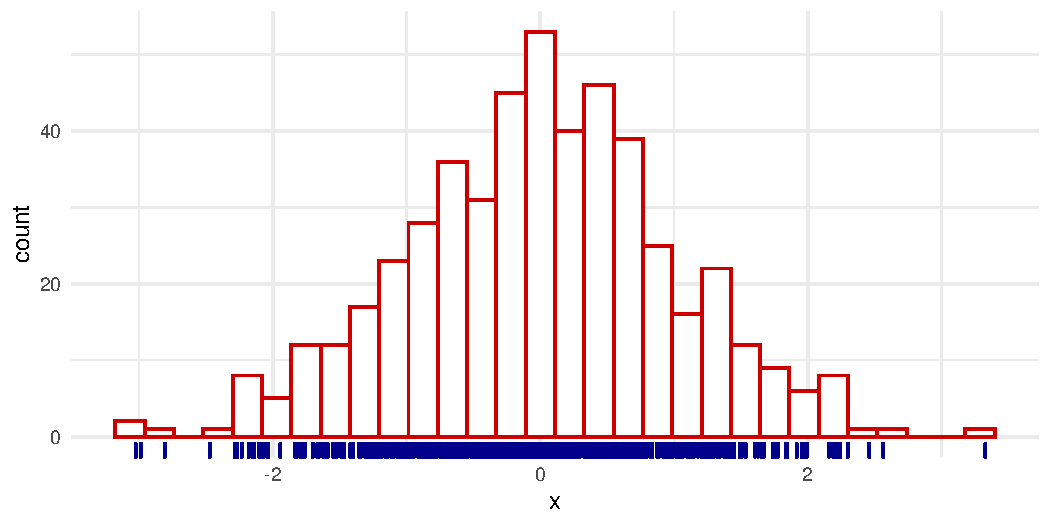
\includegraphics[width=\maxwidth]{figure/ejemplo-inicial-histograma-1} 

\end{knitrout}


\end{itemize}

Formalmente el histograma es el

\begin{equation*}
	\hat{f}_h(x) = \frac{1}{nh} \sum_{i = 1}^{n} \sum_{j} I(X_i\in B_j) I(x\in B_j),
\end{equation*}

donde \(I\) es la indicadora.

\subsection{Construcción probabilistica}

Denote \(m_j=jh-h/2\) el centro del segmento,

\begin{align*}
	\mathbb{P}\left(X\in \left[m_j - \frac{h}{2},m_j + \frac{h}{2} \right)\right) & =
	\int_{m_j - \frac{h}{2}}^{m_j + \frac{h}{2}} f(u)du                                             \\
	                                                                              & \approx f(m_j)h
\end{align*}

Esto se puede aproximar como

\begin{equation*}
	\mathbb{P} \left(X\in \left[m_j - \frac{h}{2},m_j + \frac{h}{2}\right) \right)  \approx   \frac{1}{n} \#
	\left\{X\in \left[m_j - \frac{h}{2},m_j + \frac{h}{2}\right) \right\}
\end{equation*}

Acomodando un poco la expresión

\begin{equation*}
	\hat{f}_h(m_j) =  \frac{1}{nh} \#
	\left\{X\in \left[m_j - \frac{h}{2},m_j + \frac{h}{2}\right) \right\}
\end{equation*}

\subsection{Propiedades estadísticas }

Suponga que  \(x_0 = 0\) y que \(x \in B_j\) fijo, entonces

\begin{equation*}
	\hat{f}_h(m_j) =  \frac{1}{nh} \sum_{i = 1}^{n} I(X_i \in B_j)
\end{equation*}

\subsubsection{Sesgo}

El cálculo del sesgo es el

\begin{align*}
	\mathbb{E}\left[ \hat{f}_h(m_j)\right]
	  & =  \frac{1}{nh} \sum_{i = 1}^{n} \mathbb{E}\left[ I(X_i \in B_j)\right] \\
	  & = \frac{1}{nh} n \mathbb{E}\left[ I(X_i \in B_j)\right]
\end{align*}

\(I(X_i \in B_j)\) es una indicadora con probabilidad de 1 de \(\int_{(j -
	1)h}^{jh} f(u)du\) y 0 sino.

Entonces

\begin{align*}
	\mathbb{E}\left[ I(X_i \in B_j)\right] = \mathbb{P}\left(I(X_i \in
	B_j)=1\right) = \int_{(j - 1)h}^{jh} f(u)du.
\end{align*}

Entonces,
\begin{align*}
	\mathbb{E}\left[{f}_h(m_j)\right]
	  & = \frac{1}{h} \int_{(j - 1)h}^{jh} f(u)du
\end{align*}

\begin{equation*}
	Sesgo(\hat{f}_h(m_j)) = \frac{1}{h} \int_{(j -
		1)h}^{jh} f(u)du - f(x)
\end{equation*}

Esto se puede aproximar usando Taylor alrededor del centro \(m_j = jh - h/2\) de \(B_j\) de modo que \(f(u) - f(x) \approx f^{\prime}(m_j)(u - x)\).

\begin{equation*}
	Sesgo(\hat{f}_h(m_j)) =  \frac{1}{h} \int_{(j -
		1)h}^{jh} f(u) - f(x) du \approx f^\prime(m_j)(m_j - x)
\end{equation*}

\subsubsection{Varianza}

Dado que todos los \(X_i\) son i.i.d., entonces

\begin{align*}
	\mathrm{Var}\left( \hat{f}_h(m_j)\right) & =
	\mathrm{Var}\left( \frac{1}{nh} \sum_{i = 1}^{n} I(X_i \in B_j)\right)                                  \\
	                                         & = \frac{1}{n^2h^2} n\mathrm{Var}\left( I(X_i \in B_j)\right)
\end{align*}

La variable \(I\) es una bernoulli con parametro \(\int_{(j - 1)h}^{h} f(u)du\) por lo tanto su varianza es el

\begin{equation*}
	\mathrm{Var}\left( \hat{f}_h(x)\right)\, =
	\frac{1}{nh^2} \left(\int_{(j - 1)h}^{h} f(u)du \right)\left( 1 -\int_{(j - 1)h}^{h} f(u)du \right)
\end{equation*}

\begin{tarea}{}{tarea_1}
	Usando un desarrollo de Taylor como en la parte anterior, pruebe que:
	\begin{equation*}
		\mathrm{Var}\left( \hat{f}_h(x)\right)\approx
		\frac{1}{nh} f(x)
	\end{equation*}
\end{tarea}

\subsection{Error cuadrático medio}

El error cuadrático medio del histograma es el

\begin{equation*}
	\mathrm{MSE}\left( \hat{f}_h(x)\right) =
	\mathrm{E}\left[\left(\hat{f}_h(x) - f(x)\right)^2\right] = \mathrm{Sesgo}^2\left( \hat{f}_h(x)\right) + \mathrm{Var}\left( \hat{f}_h(x)\right).
\end{equation*}

\begin{tarea}{}{tarea_2}
	¿Pueden probar la segunda igualdad de la expresión anterior?
\end{tarea}

\begin{solucion}{}{Pba_tarea2}
	Prueba segunda igualdad:
	\begin{align*}
		& \text{Sesgo}^2\left(\hat{f}_h(x)  \right) + \text{Var}\left( \hat{f}_h(x)\right)  = \\ & \left[ E\left(\hat{f}_h(x)\right) - f(x)\right]^2 + E\left[\left( E\left(\hat{f}_h(x)\right) - \hat{f}_h(x)\right)^2\right] \ =
		\\ & E\left[\left[ E\left(\hat{f}_h(x)\right) - f(x)\right]^2 + \left( E\left(\hat{f}_h(x)\right) - \hat{f}_h(x)\right)^2   \right] \ \textcolor{red}{(*)} \
	\end{align*}
	Ahora note que:
	\begin{align*}
		  & E\left[\left( E\left(\hat{f}_h(x)\right) - f(x)   \right) \left(E\left(\hat{f}_h(x)\right) - \hat{f}_h(x)    \right)    \right] \ = \                                      \\
		  & E\left[E\left(\hat{f}_h(x)\right)^2 \right] \ - \ E\left[E\left(\hat{f}_h(x)\right)\cdot \hat{f}_h(x) \right] \ - \ E\left[f(x)\cdot E\left(\hat{f}_h(x)\right)\right] \ + \\
		  & E\left[f(x)\cdot \hat{f}_h(x)\right]\ = \                                                                                                                                  \\
		  & E\left(\hat{f}_h(x)\right)^2  \ - \ E\left(\hat{f}_h(x)\right)^2  \ - \ E\left(\hat{f}_h(x)\right)\cdot E\left( f(x)\right) \ + \
		E\left( f(x)\right)\cdot E\left(\hat{f}_h(x)\right) \                                                                                                                         \\
		  & = 0
	\end{align*}
	Entonces:
	\begin{align*}
		  & \textcolor{red}{(*)} \ = \ E\left[\left[ E\left(\hat{f}_h(x)\right) - f(x)\right]^2 \ -  \right.                                                                                                         \\
		  & \left. \ 2\left( E\left(\hat{f}_h(x)\right) - f(x)   \right) \left(E\left(\hat{f}_h(x)\right) - \hat{f}_h(x)    \right) \ + \ \left( E\left(\hat{f}_h(x)\right) - \hat{f}_h(x)\right)^2   \right] \ = \  \\
		  & E\left[ \left(E\left(\hat{f}_h(x)\right) - f(x) \ - \ E\left(\hat{f}_h(x)\right) + \hat{f}_h(x) \right)^2   \right] \ = \                                                                                \\
		  & E\left[\left(\hat{f}_h(x) - f(x)\right)^2    \right]
	\end{align*}
	\qed
\end{solucion}

Retomando los términos anteriores se tiene que

\begin{multline*}
	\mathrm{MSE}\left( \hat{f}_h(x)\right) =
	\frac{1}{nh} f(x) + f^\prime
	\left\{
	\left(
	j - \frac{1}{2}
	\right) h
	\right\}^2
	\left\{
	\left(
	j - \frac{1}{2}
	\right) h - x
	\right\}^2 \\
	+ o\left(h \right) + 		o\left(\frac{1}{nh} \right)
\end{multline*}

\begin{nota}{}{}
	Si \(h \to 0\) y \(nh \to \infty\) entonces \(\mathrm{MSE}\left(  \hat{f}_h(x)\right) \to 0 \). Es decir, conforme usamos más observaciones, pero el ancho de banda de banda no decrece tan rápida, entonces el error cuadrático medio converge a 0.

	Esto indica que si \(\mathrm{MSE}\left(  \hat{f}_h(x)\right) \to 0 \) (convergencia en \(\mathbb{L}^2\)) implica que \(\hat{f}_h(x) \stackrel{\mathcal{P}}{\to} f(x)\), por lo tanto \(\hat{f}_h\) es consistente.
\end{nota}

La fórmula anterior tiene la siguiente particularidad

\begin{itemize}
	\item Si \(h\to 0\), la varianza crece (converge a \(\infty\)) y el sesgo decrece (converge a \(f^\prime (0)x^2\)).
	\item Si \(h\to \infty\), la varianza decrece (hacia 0)  y el sesgo crece (hacia \(\infty\))
\end{itemize}

Note que la figura \ref{fig:MSE-histograma}




\begin{knitrout}
\definecolor{shadecolor}{rgb}{1, 1, 1}\color{fgcolor}
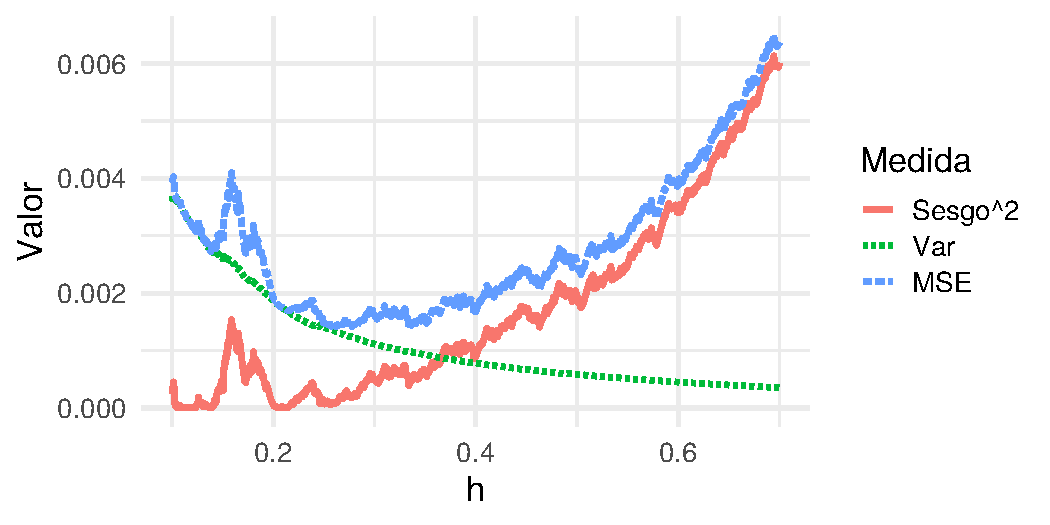
\includegraphics[width=\maxwidth]{figure/MSE-histograma-1} 

\end{knitrout}


\subsection{Error cuadrático medio integrado}

El problema con el \(\mathrm{MSE}\left(  \hat{f}_h(x)\right)\) es que depende completamente del punto escogido \(x\).

La solución a esto es integrar el MSE.

\begin{align*}
	\mathrm{MISE}\left(  \hat{f}_h(x)\right)
	  & = \mathrm{E}\left[
		\int_{ -\infty}^{\infty} \left\{
		\hat{f}_h(x) - f(x)
		\right\}^2 dx
		\right]                                                       \\
	  & = \int_{ -\infty}^{\infty} \mathrm{E}\left[
		\left\{
		\hat{f}_h(x) - f(x)
		\right\}^2
		\right] dx                                                    \\
	  & = \int_{ -\infty}^{\infty}\mathrm{MSE}(\hat{f}_h(x)) \, dx
\end{align*}

Además,

\begin{align*}
	\mathrm{MISE} (\hat{f}_h(x))
	  & = \int_{ -\infty}^{\infty} \frac{1}{nh} f(x)dx                                                                                                                                          \\
	  & + \int_{ -\infty}^{\infty}\, \sum_{j}^{} I(x\in B_j) \left\{ \left( j- \frac{1}{2} \right)h -x  \right\}^2 \left [f^\prime \left( \left\{j - \frac{1}{2}\right\}h \right)  \right]^2 dx \\
	  & = \frac{1}{nh} + \sum_{j}^{} \left [f^\prime \left( \left\{j - \frac{1}{2}\right\}h \right)  \right]^2 \int_{ B_j}    \left\{ \left( j- \frac{1}{2} \right)h -x  \right\}^2 dx          \\
	  & =\frac{1}{nh} + \frac{h^2}{12} \sum_{j} \left [f^\prime \left( \left\{j - \frac{1}{2}\right\}h \right)  \right]^2                                                                       \\
	  & \approx \frac{1}{nh} + \frac{h^2}{12} \int \{f^\prime(x)\}^2 dx                                                                                                                         \\
	  & =\frac{1}{nh} + \frac{h^2}{12} \Vert f^\prime\Vert_{2}^2
\end{align*}

\subsection{Ancho de banda óptimo para el histograma}

El MISE tiene el mismo comportamiento que el MSE. Figura \ref{fig:MISE-histograma} presenta el comportamiento de la varianza, sesgo y MISE para nuestro ejemplo.

\begin{knitrout}
\definecolor{shadecolor}{rgb}{1, 1, 1}\color{fgcolor}\begin{figure}
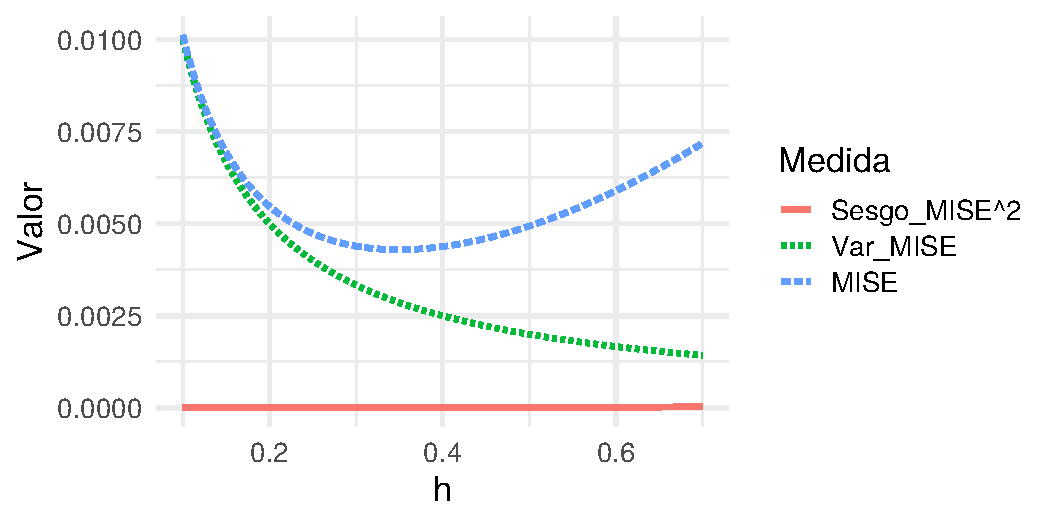
\includegraphics[width=\maxwidth]{figure/MISE-histograma-1} \caption[ ]{ }\label{fig:MISE-histograma}
\end{figure}


\end{knitrout}


La mala elección del parámetro $h$ causa que el histograma no capture toda la estructura de los datos.

\begin{knitrout}
\definecolor{shadecolor}{rgb}{1, 1, 1}\color{fgcolor}
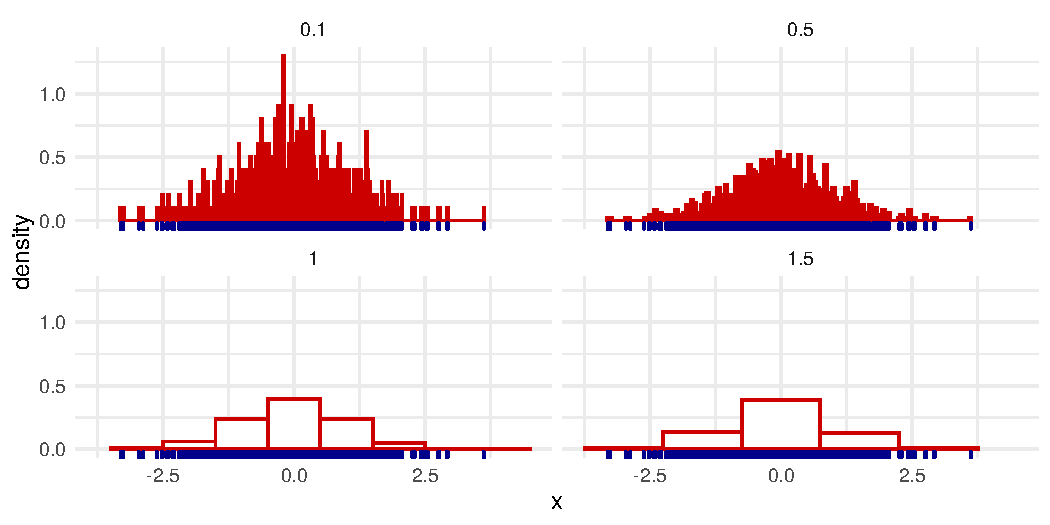
\includegraphics[width=\maxwidth]{figure/unnamed-chunk-4-1} 

\end{knitrout}


En este caso se puede simplemente minimizar el MISE de la forma usual,

\begin{equation*}
	\frac{\partial \mathrm{MISE}(f_{h})}{\partial h} = -\frac{1}{nh^2} + \frac{1}{6} h \Vert f^\prime\Vert_{2}^2 = 0
\end{equation*}

implica que

\begin{equation*}
	h_{opt} = \left(\frac{6}{n\Vert f^\prime\Vert_{2}^2}\right) ^{1/3} = O\left( n^{1/3} \right).
\end{equation*}

y que por lo tanto

\begin{equation*}
	\mathrm{MISE}(\hat{f}_{h}) = \frac{1}{n} \left(\frac{n\Vert f^\prime\Vert_{2}^2}{6}\right)  ^{1/3}
\end{equation*}

\begin{nota}{Recuerde de Estadística I}{}

	Si \(X_1, \ldots, X_2 \sim f_{\theta} \) i.i.d, con \(\mathrm{Var}(X) = \sigma^2\), recuerde que el estimador \(\hat{\theta}\)  de \(\theta\) tiene la característica que

	\begin{equation*}
		\mathrm{MSE}(\theta) = \mathrm{Var}(\hat{\theta}) +
		\mathrm{Sesgo}^2(\hat{\theta}) = \frac{\sigma^2}{n}
	\end{equation*}
\end{nota}

Según la nota anterior la tasas de convergencia del histograma es más lenta que la de un estimador parámetrico considerando la misma cantidad de datos.

\begin{knitrout}
\definecolor{shadecolor}{rgb}{1, 1, 1}\color{fgcolor}
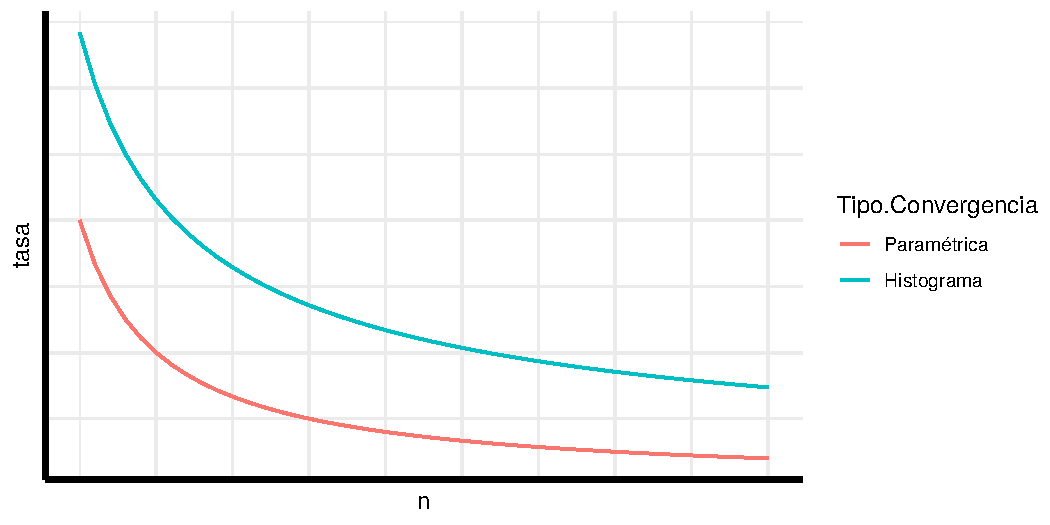
\includegraphics[width=\maxwidth]{figure/unnamed-chunk-5-1} 

\end{knitrout}





Finalmente, podemos encontrar el valor óptimo  de esta datos dado por $h=0.334$
\begin{knitrout}
\definecolor{shadecolor}{rgb}{1, 1, 1}\color{fgcolor}
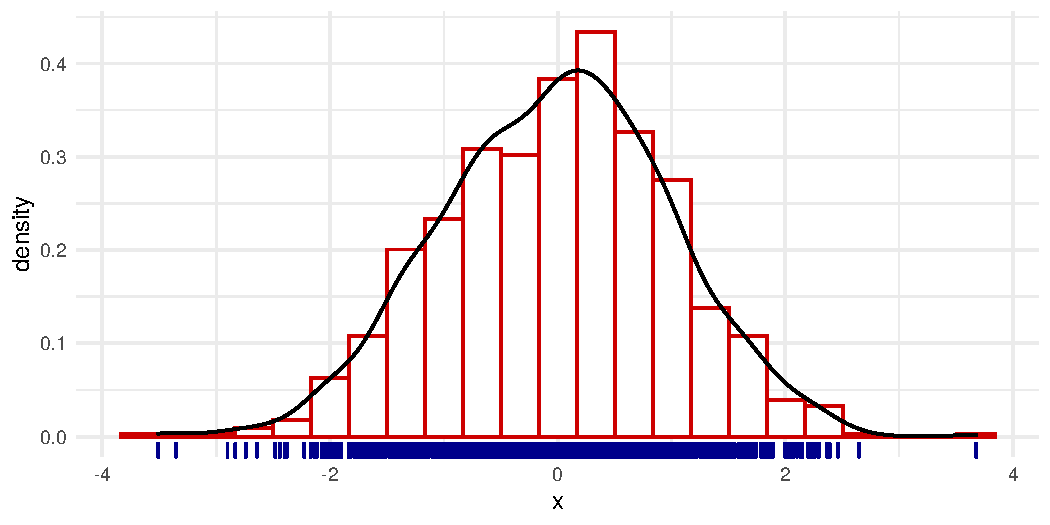
\includegraphics[width=\maxwidth]{figure/unnamed-chunk-7-1} 

\end{knitrout}




\newpage

\section{Estimación No-paramétrica de densidad}

\subsection{Primera construcción}

Sea $X_{1},\ldots,X_{n}$ variables aleatorias i.i.d. con distribución $f$ en $\mathbb{R}$.

La distribución de  $f$ es  $F(x)=\int_{-\infty}^{x}f(t)dt$.

Considere la distribución empírica como
\[
	F_{n}(x)=\frac{1}{n}\sum_{i=1}^{n}I(X_{i}\leq x).
\]

Por la ley de los grandes números tenemos que \(\hat{F}_{n}(x)
\xrightarrow{c.s} F(x)\) para todo  $x$ en $\mathbb{R}$as
$n\rightarrow\infty$. Entonces, $F_{n}(x)$ es consistente

para todo $x$ in $\mathbb{R}$.

\begin{pregunta}{}{}
	?`Podríamos derivar \(\hat{F}_n\) para encontrar el estimar \(\hat{f}_n\)?
\end{pregunta}

La respuesta es si (más o menos).
\newpage
Suponga que $h>0$ tenemos la aproximación
\[
	f(x)\approx\frac{F(x+h)-F(x-h)}{2h}.
\]

Remplazando $F$  por su estimador  $\hat{F}_{n}$, defina
\[
	\hat{f}_{n}^{R}(x)=\frac{F_{n}(x+h)-F_{n}(x-h)}{2h},
\]
donde $\hat{f}_{n}^{R}(x)$ es el estimador de \emph{Rosenblatt }.

Podemos rescribirlo de la forma,
\[
	\hat{f}_{n}^{R}(x)=\frac{1}{2nh}\sum_{i=1}^{n}I(x-h<X_{i}\leq x+h)=\frac{1}{nh}\sum_{i=1}^{n}K_{0}\left(\frac{X_{i}-x}{h}\right)
\]
con  $K_{0}(u)=\frac{1}{2}I(-1<u\leq1)$, lo cuál es equivalente al caso del histograma.

\newpage

\subsection{Otra construcción}

Con el histograma construimos una serie de segmentos fijo \(B_{j}\) y contabamos el número de datos que estaban \textbf{CONTENIDOS} en \(B_{j}\)

\begin{pregunta}{}{}
	¿Qué pasaría si cambiamos la palabra \textbf{CONTENIDOS} por \textbf{ALREDEDOR DE ``x''}?
\end{pregunta}

Suponga que se tienen intervalos de longitud $ 2h $, es decir, intervalos de la forma $ [x-h,x+h) $.

El histograma  se escribe como

\begin{equation*}
	\hat{f_{h}}(x) = \dfrac{1}{2hn} \# \{ X_i \in [x-h,x+h) \}.
\end{equation*}

Ahora tratemos de modificar ligeramente esta expresión notando dos cosas

\begin{enumerate}
	\item \begin{equation*}
		      \frac{1}{2} I \left( \left\vert u \right\vert \leq 1 \right)
	      \end{equation*}
	      con \(u = \frac{x-xi}{h}\)
	\item

	      \begin{equation*}
		      \frac{1}{2}\# \{ X_i \in [x-h,x+h) \}
		      =\sum_{i=1}^{n} K\left( \frac{x-x_{i}}{h} \right)
		      =\sum_{i=1}^{n}  \frac{1}{2} I \left( \left\vert \frac{x-x_{i}}{h}
		      \right\vert \leq 1 \right)
	      \end{equation*}
\end{enumerate}

Finalmente se tiene que

\begin{equation*}
	\hat{f}_{h}\left( x \right) = \frac{1}{nh}\sum_{i=1}^{n} K\left( \frac{x-x_{i}}{h} \right)
\end{equation*}

\begin{center}
	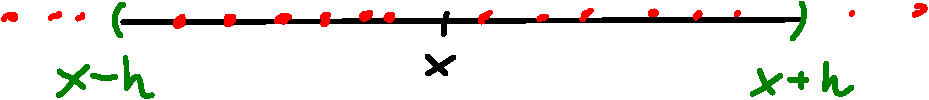
\includegraphics[width=\linewidth]{manual_figure/np-density-interval-crop.pdf}
\end{center}

\newpage
\begin{pregunta}{}{}
	¿Qué pasaría si cambiaríamos la función \(K\) del histograma por una más general?
\end{pregunta}

Esta función debería cumplir las siguientes características

\begin{itemize}
	\item \(K(u)\geq 0\).
	\item \(\int_{-\infty}^{\infty} K(u)du = 1 \).
	\item \(\int_{-\infty}^{\infty} u K(u)du = 0\).
	\item \(\int_{-\infty}^{\infty} u^{2} K(u)du <\infty\).
\end{itemize}

Por ejemplo:

\begin{description}
	\item[Uniforme:] \(\frac{1}{2} I \left( \left\vert u \right\vert \leq 1 \right)\).
	\item[Triangular:] \( (1-|u|) I \left( \left\vert u \right\vert \leq 1 \right)\).
	\item[Epanechnikov:] \(\frac{3}{4} (1-u^{2}) I \left( \left\vert u \right\vert \leq 1 \right)\).
	\item[Gausian:] \(\frac{1}{\sqrt{2\pi}} \exp \left( -\frac{1}{2}u^{2} \right)\).
\end{description}

\begin{knitrout}
\definecolor{shadecolor}{rgb}{1, 1, 1}\color{fgcolor}
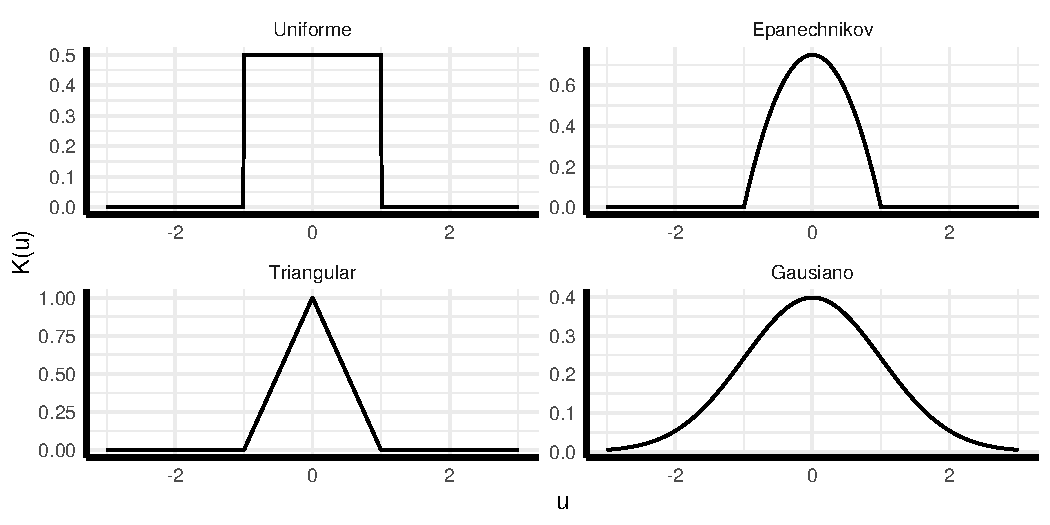
\includegraphics[width=\maxwidth]{figure/unnamed-chunk-9-1} 

\end{knitrout}


Entonces se tendría que la expresión general para un estimador por núcleos es

\begin{equation*}
	\hat{f}_{h}\left( x \right) = \frac{1}{nh}\sum_{i=1}^{n} K\left( \frac{x-x_{i}}{h} \right)
\end{equation*}

\newpage

\begin{pregunta}{}{}
	¿Qué pasaría si modificamos el ancho de banda \(h\) para un mismo kernel?
\end{pregunta}

Nuevamente sería el ancho de banda ya que

\begin{knitrout}
\definecolor{shadecolor}{rgb}{1, 1, 1}\color{fgcolor}
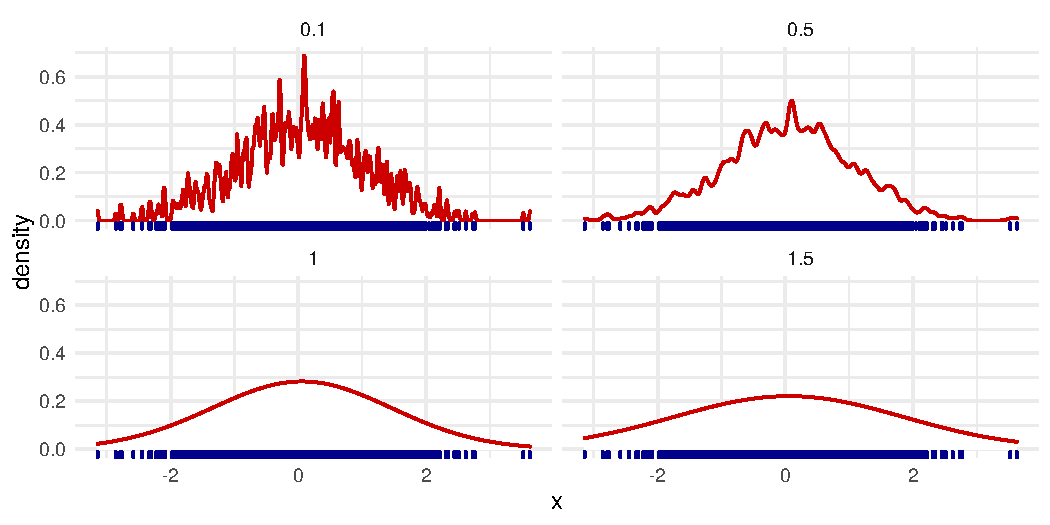
\includegraphics[width=\maxwidth]{figure/unnamed-chunk-10-1} 

\end{knitrout}


\newpage

\begin{pregunta}{}{}
	¿Qué pasaría si modificamos el kernel para un mismo ancho de banda \(h\)?
\end{pregunta}

\begin{knitrout}
\definecolor{shadecolor}{rgb}{1, 1, 1}\color{fgcolor}
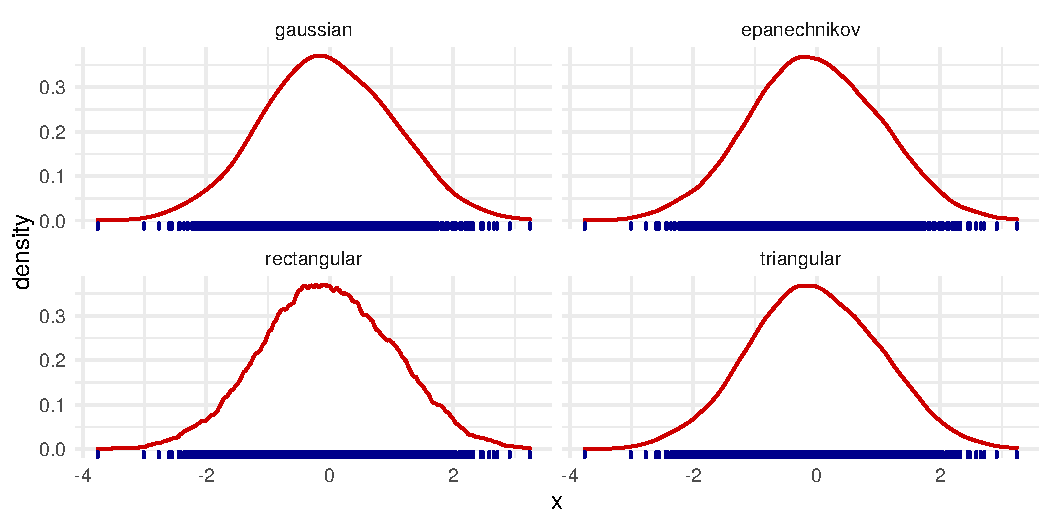
\includegraphics[width=\maxwidth]{figure/unnamed-chunk-11-1} 

\end{knitrout}


\newpage

Recordemos nuevamente la fórmula

\begin{equation*}
	\hat{f}_{h}\left( x \right) = \frac{1}{nh}\sum_{i=1}^{n} K\left( \frac{x-X_{i}}{h} \right)
\end{equation*}

Cada sumando de esta expresión es una función por si misma. Si la integramos se obtiene que

\begin{equation*}
	\frac{1}{nh}\int K\left( \frac{x-X_{i}}{h} \right) dx
	= \frac{1}{nh} \int K\left( u \right) h du
	= \frac{1}{n} \int K(u) du
	= \frac{1}{n}
\end{equation*}

\begin{knitrout}
\definecolor{shadecolor}{rgb}{1, 1, 1}\color{fgcolor}
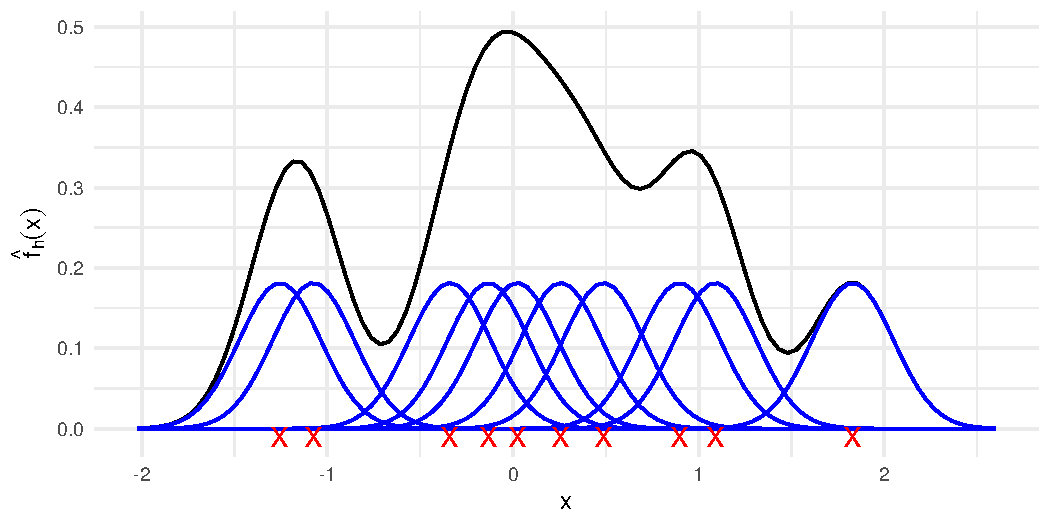
\includegraphics[width=\maxwidth]{figure/unnamed-chunk-12-1} 

\end{knitrout}


\newpage

\subsection{Propiedades Estadísticas}

\begin{pregunta}{}{}
	¿Podríamos imitar lo mismo que hicimos para el histograma?
\end{pregunta}

Si. Las propiedades que vimos anteriormente son universales para estimadores.

Entonces:
\begin{align*}
	\mathrm{MSE}(\hat{f}_{h}(x)) & =\mathrm{Var}(\hat{f}_{h}(x))+\mathrm{Sesgo}^{2} (\hat{f}_{h}(x))            \\
	\mathrm{MISE}(\hat{f}_{h})   & =\int\mathrm{Var}(\hat{f}_{h}(x))dx+\int\mathrm{Sesgo}^{2}(\hat{f}_{h}(x))dx
\end{align*}

donde

\(\mathrm{Var}\left(\hat{f}_{h}(x)\right)=\mathbb{E}\left[\hat{f}_{h}(x)-\mathbb{E}\hat{f}_{h}(x)\right]^{2}\) and \(\mathrm{Sesgo}\left(\hat{f}_{h}(x)\right)=\mathbb{E}\left[\hat{f}_{h}(x)\right]-f(x)\).

\newpage

\subsubsection{Varianza}

\begin{align*}
	\mathrm{Var}(\hat{f}_{h}(x))
	  & =\mathrm{Var}\left(\frac{1}{n}\sum_{i=1}^{n}K\left(\frac{x-X_{i}}{h}\right)\right)          \\
	  & =\frac{1}{n^{2}h^{2}}\sum_{i=1}^{n}\mathrm{Var}\left(K\left(\frac{x-X_{i}}{h}\right)\right) \\
	  & =\frac{1}{nh^{2}}\mathrm{Var}\left(K\left(\frac{x-X}{h}\right)\right)                       \\
	  & =\frac{1}{nh^{2}}\left\{
	\textcolor{red}{\mathbb{E}\left[K^{2}\left(\frac{x-X}{h}\right)\right]}
	-\left\{
	\textcolor{blue}{\mathbb{E}\left[K\left(\frac{x-X}{h}\right)\right]}
	\right\}^{2}
	\right\}.
\end{align*}
Usando que:
\begin{align*}
	\textcolor{red}{\mathbb{E}\left[K^{2}\left(\frac{x-X}{h}\right)\right]}
	  & =\int K^{2}\left(\frac{x-s}{h}\right)f(s)ds            \\
	  & =h\int K^{2}\left(u\right)f(uh+x)du                    \\
	  & =h\int K^{2}\left(u\right)\left\{ f(x)+o(1)\right\} du \\
	  & =h\left\{ \Vert K\Vert_{2}^{2}f(x)+o(1)\right\} .
\end{align*}

\begin{align*}
	\textcolor{blue}{\mathbb{E}\left[K\left(\frac{x-X}{h}\right)\right]}
	  & =\int K\left(\frac{x-s}{h}\right)f(s)ds            \\
	  & =	h\int K\left(u\right)f(uh+x)du                    \\
	  & =h\int K\left(u\right)\left\{ f(x)+o(1)\right\} du \\
	  & =h\left\{f(x)+o(1)\right\} .
\end{align*}

Por lo tanto se obtiene que

\begin{equation*}
	\mathrm{Var}\left(\hat{f}_{h}(x)\right) = \frac{1}{nh} \Vert K\Vert_{2}^{2}f(x) + o\left(\frac{1}{nh}\right), \text{ si } nh\to \infty.
\end{equation*}

\newpage

\subsubsection{Sesgo}

Para el sesgo tenemos

\begin{align*}
	\mathrm{Sesgo}\left(\hat{f}_{h}(x)\right)
	  & = \mathbb{E}\left[\hat{f}_{h}(x)\right]-f(x)                                                  \\
	  & = \frac{1}{nh} \sum_{i=1}^{n} \mathrm{E}\left[K\left( \frac{x-X_{i}}{h} \right)\right] - f(x) \\
	  & = \frac{1}{h}\mathrm{E}\left[K\left( \frac{x-X_{1}}{h} \right)\right] - f(x)                  \\
	  & = \int \frac{1}{h} K\left( \frac{x-u}{h}\right)f(u)du -f(x)                                   \\
\end{align*}

\begin{tarea}{}{}
	Usando el cambio de variable \(s=\frac{u-x}{h}\) y las propiedades del kernel pruebe que

	\begin{equation*}
		\mathrm{Sesgo}\left(\hat{f}_{h}(x)\right) = \frac{h^{2}}{2} f^{\prime\prime} \mu_{2}(K) + o(h^{2}), \text{ si } h\to 0
	\end{equation*}
	donde \(\mu_{2}=\int s^{2}K(s)ds\).

	\emph{\textbf{Nota:} En algunas pruebas más formales, se necesita
	además que  $f^{\prime\prime}$ sea absolutamente continua y que
	$\int(f^{\prime\prime\prime}(x))dx<\infty$.}
\end{tarea}

\begin{solucion}{}{Pba_tarea_Sesgo}
	\begin{align*}
\mathrm{Sesgo}(\hat{f_{h}}(x)) & = \int \frac{1}{h} K\left( \frac{x-u}{h} \right) f(u)du - f(x)		\\
& = \frac{1}{h} \int hK(s)f(sh+x) ds - f(x) \\
 & = \int K(s)\Biggl[ f(x) + f^{\prime}(x)(sh+x-x)  \\
 &  \qquad  + \frac{f^{\prime\prime}(x)}{2}(sh+x-x)^2 + o(h^{2}) \Biggr] - f(x) \\
 & = \int K(s)f(x)ds + \int hf^{\prime}(x)sK(s) ds  \\
 & \qquad  + \int \frac{h^2}{2} f^{\prime\prime}(x)s^2K(s) ds + o(h^2) - f(x) \\
 & = f(x) + 0 + \frac{h^2}{2}f^{\prime\prime}(x)\mu_{2}(K) + o(h^2) - f(x)	\\
 & = \frac{h^2}{2}f^{\prime\prime}(x)\mu_{2}(K) + o(h^2) \\
	\end{align*}
\end{solucion}

\begin{knitrout}
\definecolor{shadecolor}{rgb}{1, 1, 1}\color{fgcolor}
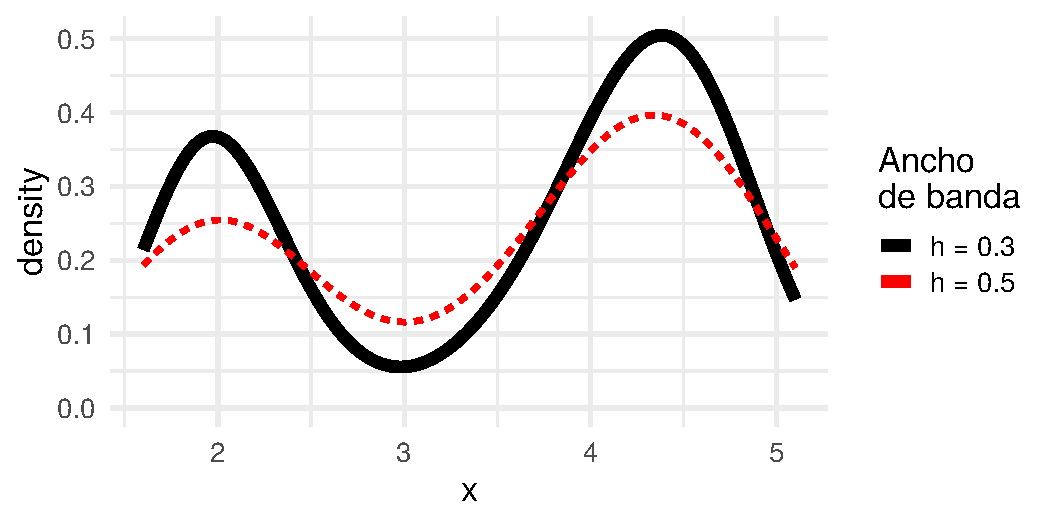
\includegraphics[width=\maxwidth]{figure/unnamed-chunk-13-1} 

\end{knitrout}


\begin{nota}{}{}
	Note como los cambios en el ancho de banda modifican la suavidad (sesgo) y el aplanamiento de la curva (varianza).
\end{nota}

\newpage

\subsubsection{Error cuadrático medio y Error cuadrático medio integrado}

El error cuadrático medio se escribe
\begin{align*}
	\mathrm{MSE}(\hat{f}_{h}(x))
	  & = \mathrm{Sesgo}\left(\hat{f}_{h}(x)\right)^{2} + \mathrm{Var}\left(\hat{f}_{h}(x)\right)                                                 \\
	  & = \frac{h^{4}}{4}\left(\mu_{2}(K)f^{\prime\prime}(x)\right)^{2}+\frac{1}{nh}\Vert K\Vert_{2}^{2}f(x)+o(h^{4})+o\left(\frac{1}{nh}\right).
\end{align*}

Y el error cuadrático medio integrado se escribe como,
\begin{align*}
	\mathrm{MISE}\left(\hat{f}_{h}\right) & = \int \mathrm{MSE}\left(\hat{f}_{h}(x)\right)dx                                                                                                        \\
	                                      & = \int \mathrm{Sesgo}\left(\hat{f}_{h}(x)\right)^{2} + \mathrm{Var}\left(\hat{f}_{h}(x)\right)dx                                                        \\
	                                      & = \frac{h^{4}}{4}\mu_{2}^{2}(K)\left\Vert f^{\prime\prime}(x)\right\Vert_{2}^{2} +\frac{1}{nh}\Vert K\Vert_{2}^{2}+o(h^{4})+o\left(\frac{1}{nh}\right).
\end{align*}
\newpage
\subsubsection{Ancho de banda óptimo}

Minimizando el \(\mathrm{MISE}\) con respecto a \(h\) obtenemos
\begin{equation*}
	h_{opt}=\left(\frac{\Vert K\Vert_{2}^{2}}{\Vert f^{\prime\prime}\Vert_{2}^{2}\left(\mu_{2}(K)\right)^{2}n}\right)^{1/5}=O\left( n^{-1/5} \right).
\end{equation*}

\begin{nota}{}{}
	De forma práctica, $h_{opt}$ no es un estimador útil de $h$ porque depende de $\Vert f^{\prime\prime}\Vert_{2}^{2}$  que es desconocido.

	Más adelante veremos otra forma de encontrar este estimador.
\end{nota}

Evaluando $h_{opt}$ en el \(\mathrm{MISE}\) tenemos que

\begin{equation*}
	\mathrm{MISE}(\hat{f}_{h})=\frac{5}{4}\left(\Vert K\Vert_{2}^{2}\right)^{4/5}\left(\Vert f^{\prime\prime}\Vert_{2}^{2}\mu_{2}(K)\right)^{2/5}n^{-4/5} = O\left( n^{-4/5} \right).
\end{equation*}

\begin{knitrout}
\definecolor{shadecolor}{rgb}{1, 1, 1}\color{fgcolor}
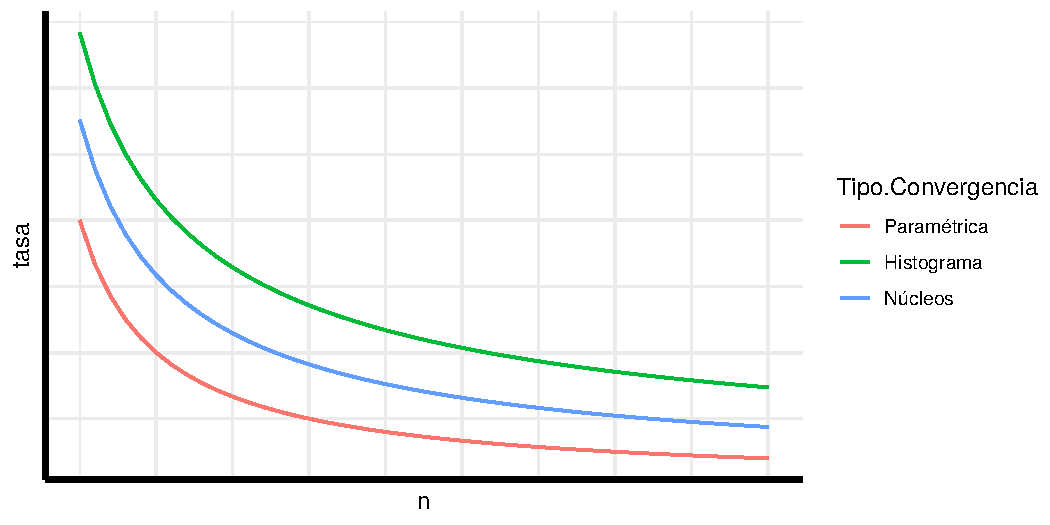
\includegraphics[width=\maxwidth]{figure/unnamed-chunk-14-1} 

\end{knitrout}


\newpage

\begin{nota}{Detalle técnico}{}
	Formalmente, es posible probar que si $f$ es $\beta$ veces continuamente diferenciable y  $\int\left(f^{(\beta)}\right)^{2}<\infty$, entonces se tiene que
	\[
		{\displaystyle h_{opt}=O\left(n^{-\frac{1}{2\beta+1}}\right).}
	\]
	Por lo tanto se podría aproximar a una tasa paramétrica de convergencia si
	\(\beta\) es grande.
\end{nota}

\newpage

\subsection{Escogiendo el ancho de banda}

\begin{nota}{}{}
	La principal característica del ancho de banda
	\begin{equation*}
		h_{opt}=\left(\frac{\Vert K\Vert_{2}^{2}}{\Vert f^{\prime\prime}\Vert_{2}^{2}\left(\mu_{2}(K)\right)^{2}n}\right)^{1/5}=O\left( n^{-1/5} \right).
	\end{equation*}

	ES QUE ¡NO FUNCIONA!

\end{nota}

Veremos dos métodos para determinar un \(h\) que funcione:

\begin{itemize}
	\item Referencia normal.
	\item Validación cruzada.
\end{itemize}

\newpage

\subsubsection{Referencia normal}

\begin{cuidado}{}{}
	Este método es más efectivo si se conoce que la verdadera distribución es bastante suave, unimodal y simétrica.

	Más adelante veremos otro método para densidades más generales.
\end{cuidado}

Asuma que \(f\) es normal distribuida y se utiliza un kernel \(K\) gausiano. Entonces se tiene que

\begin{align*}
	\hat{h}_{rn} & =\left(\frac{\Vert K\Vert_{2}^{2}}{\Vert f^{\prime\prime}\Vert_{2}^{2}\left(\mu_{2}(K)\right)^{2}n}\right)^{1/5}=O\left( n^{-1/5} \right) \\
	             & =1.06 \hat{\sigma} n^{-1/5}.
\end{align*}

donde

\begin{equation*}
	\hat{\sigma} = \sqrt{\frac{1}{n-1} \sum_{i=1}^{n} \left( x_{i}-\bar{x}^{2} \right)}
\end{equation*}

\begin{tarea}{}{}
	Pruebe que la ecuación anterior es verdadera. Es decir, calcule \(\Vert K\Vert_{2}^{2}\), \(\Vert f^{\prime\prime}\Vert_{2}^{2}\) y \(\mu_{2}(K)\)
\end{tarea}

\begin{nota}{}{}
	Un problema con \(\hat{h}_{rn}=1.06 \hat{\sigma} n^{-1/5}\) es su sensibilidad a los valores extremos.
\end{nota}

\begin{ejemplo}{}{}
	La varianza empírica de  1, 2, 3, 4, 5, es  2.5.

	La varianza empírica de 1, 2, 3, 4, 5, 99, es 1538.
\end{ejemplo}

El rango intercuantil IQR se define como
\begin{equation*}
	\mathrm{IQR}^{X} = Q^{X}_{3} - Q^{X}_{1}
\end{equation*}
donde \(Q^{X}_{1}\) y \(Q^{X}_{3}\) son el primer y tercer  de un conjunto de datos \(X_{1},\ldots, X_n\).

Con el supuesto que \(X\sim \mathcal{N}(\mu,\sigma^{2})\) entonces \(\displaystyle Z = \frac{X-\mu}{\sigma} \sim \mathcal{N}(0,1)\).

Entonces,
\begin{align*}
	\mathrm{IQR}
	  & = Q^{X}_{3} - Q^{X}_{1}                                                     \\
	  & = \left( \mu+\sigma Q^{Z}_{3} \right) - \left( \mu+\sigma Q^{Z}_{1} \right) \\
	  & = \sigma \left(Q^{Z}_{3} - Q^{Z}_{1} \right)                                \\
	  & \approx \sigma \left( 0.67 - (0.67) \right)                                 \\
	  & =1.34 \sigma.
\end{align*}

Por lo tanto \(\displaystyle \hat{\sigma} = \frac{\widehat{\mathrm{IQR}}^{X}}{1.34}\)

Podemos sustituir la varianza empírica de la fórmula inicial y tenemos
\begin{equation*}
	\hat{h}_{rn} = 1.06 \frac{\widehat{\mathrm{IQR}}^{X}}{1.34} n^{-\frac{1}{5}} \approx 0.79\  \widehat{\mathrm{IQR}}^{X}\ n^{-\frac{1}{5}}
\end{equation*}

Combinando ambos estimadores, podemos obtener,

\begin{equation*}
	\hat{h}_{rn} = 1.06 \min \left\{\frac{\widehat{\mathrm{IQR}}^{X}}{1.34}, \hat{\sigma }\right\} n^{-\frac{1}{5}}
\end{equation*}

\newpage

\subsubsection{Validación Cruzada}

Defina el \emph{error cuadrático integrado} como
\begin{align*}
	\mathrm{ISE}(\hat{f}_{h}) & =\int\left(\hat{f}_{h}(x)-f(x)\right)^{2}dx\nonumber                   \\
	                          & =\int \hat{f}_{h}^{2}(x)dx-2\int \hat{f}_{h}(x)f(x)dx+\int f^{2}(x)dx.
\end{align*}

\begin{nota}{}{}
	El MISE es el valor esperado del ISE.
\end{nota}

Nuestro objetivo es minimizar el ISE con respecto a \(h\).

Primero note que \(\int f^{2}(x)dx\) NO DEPENDE de \(h\). Podemos minimizar la expresión
\begin{equation*}
	\mathrm{ISE}(\hat{f}_{h})-\int f^{2}(x)dx=
	\textcolor{red}{\int\hat{f}_{h}^{2}(x)dx}
	-2
	\textcolor{blue}{\int\hat{f}_{h}(x)f(x)dx}
\end{equation*}

Vamos a resolver esto en dos pasos partes

\newpage

\paragraph{ Integral \(\textcolor{blue}{\int\hat{f}_{h}(x)f(x)dx}\)}  \ \newline

El término \(\textcolor{blue}{\int\hat{f}_{h}(x)f(x)dx}\) es el valor esperado de
\(\mathrm{E}\left[\hat{f}(X)\right]\). Su estimador es
\begin{equation*}
	\widehat{\mathrm{E}\left[\hat{f}(X)\right]}
	= \frac{1}{n}\sum_{i=1}^{n}\hat{f}_{h}(X_{i})
	=\frac{1}{n^{2}h}\sum_{i=1}^{n}\sum_{j=1}^{n}
	K\left(\frac{X_{j}-X_{i}}{h}\right).
\end{equation*}

\begin{cuidado}{}{}
	El problema con esta expresión es que las observaciones que se usan para estimar la esperanza son las misma que se usan para estimar \(\hat{f}_{h}(x)\) (Se utilizan doble).
\end{cuidado}

La solución es remover la  $i^{\text{ésima}}$ observación de $\hat{f}_{h}$ para cada \(i\).

Redefiniendo el estimador anterior tenemos $\int \hat{f}_{h}(x)f(x)dx$ como
\[
	\frac{1}{n}\sum_{i=1}^{n}\hat{f}_{h,-i}(X_{i}),
\]
donde
\[
	\hat{f}_{h,-i}(x)=\frac{1}{(n-1)h}\sum_{\substack{j=1\\ j\neq i}}^{n}K\left( \frac{x-X_{i}}{h} \right) .
\]
\newpage

\paragraph{ Integral \(\textcolor{red}{\int\hat{f}_{h}^{2}(x)dx}\)}  \ \newline

Siguiendo con el término \(\textcolor{red}{\int\hat{f}_{h}^{2}(x)dx}\) note que este se puede reescribir como

\begin{align*}
	\textcolor{red}{\int\hat{f}_{h}^{2}(x)dx}
	  & =\int\left(\frac{1}{nh}\sum_{i=1}^{n}K\left( \frac{x-X_{i}}{h} \right)\right)^{2}dx                                    \\
	  & =\frac{1}{n^{2}h^{2}}\sum_{i=1}^{n}\sum_{i=1}^{n}\int K\left(\frac{x-X_{i}}{h}\right)K\left(\frac{x-X_{j}}{h}\right)dx \\
	  & =\frac{1}{n^{2}h}\sum_{i=1}^{n}\sum_{i=1}^{n}\int K\left(u\right)K\left(\frac{X_{i}-X_{j}}{h}-u\right)du               \\
	  & =\frac{1}{n^{2}h}\sum_{i=1}^{n}\sum_{i=1}^{n}K*K\left(\frac{X_{i}-X_{j}}{h}\right).
\end{align*}

donde $K*K$ es la convolución de  $K$  consigo misma.

\newpage
Finalmente tenemos la  función,

\[
	\mathrm{CV}(h)=\frac{1}{n^{2}h}\sum_{i=1}^{n}\sum_{j=1}^{n}K*K\left(\frac{X_{i}-X_{j}}{h}\right)-\frac{2}{(n-1)h}\sum_{i=1}^{n}\mathop{\sum_{j=1}^{n}}_{j\neq i}K\left( \frac{X_{i}-X_{j}}{h} \right).
\]

\begin{nota}{}{}
	Note que \(\mathrm{CV}(h)\) no depende de \(f\) o sus derivadas.
\end{nota}

\begin{nota}{}{}
	Para efectos prácticos es mejor utilizar el criterio

	\[
		CV(h)=\int\hat{f}_{h}^{2}(x)dx-\frac{2}{(n-1)h}\sum_{i=1}^{n}\mathop{\sum_{j=1}^{n}}_{j\neq i}K\left( \frac{X_{i}-X_{j}}{h} \right)
	\]
	y luego calcular numéricamente la integral.
\end{nota}

\newpage

\subsection{Intervalos de confianza para estimadores de densidad no paramétricos}

Usando los resultados anteriores y asumiendo que \(h=cn^{-\frac{1}{5}}\) entonces

\begin{equation*}
	n^{-\frac{2}{5}} \left\{ \hat{f}_{h}(x) -f(x)\right\}
	\xrightarrow{\mathcal{L}} \mathcal{N}\left(\underbrace{\frac{c^{2}}{2} f^{\prime\prime}
		\mu_{2}(K)}_{b_{x}}, \underbrace{\frac{1}{c}f(x) \left\Vert K \right\Vert_{2}^{2}}_{v_{x}}\right).
\end{equation*}

Si \(z_{1-\frac{\alpha}{2}}\) es el cuantil \(1-\frac{\alpha}{2}\) de una distribución normal estándar, entonces

\begin{align*}
	1-\alpha
	  & \approx \mathbb{P}\left(b_{x}-z_{1-\frac{\alpha}{2}} v_{x} \leq n^{2 / 5}\left\{\widehat{f}_{h}(x)-f(x)\right\} \leq b_{x}+z_{1-\frac{\alpha}{2}} v_{x}\right) \\
	  & =\mathbb{P}\left(\widehat{f}_{h}(x)-n^{-2 / 5}\left\{b_{x}+z_{1-\frac{\alpha}{2}} v_{x}\right\}\right.                                                         \\
	  & \qquad\qquad \left. \leq f(x)\leq \hat{f}_{h}(x)-n^{-2 / 5}\left\{b_{x}-z_{1-\frac{\alpha}{2}} v_{x}\right\}\right)
\end{align*}

Esta expresión nos dice que con una probabilidad de  \(1-\alpha\) se tiene que

\begin{equation*}
	\begin{aligned}
		  & \left[\hat{f}_{h}(x)-\frac{h^{2}}{2} f^{\prime \prime}(x) \mu_{2}(K)-z_{1-\frac{\alpha}{2}} \sqrt{\frac{f(x)\|K\|_{2}^{2}}{n h}}\right. \\
		  & \left.\widehat{f}_{h}(x)-\frac{h^{2}}{2} f^{\prime \prime}(x) \mu_{2}(K)+z_{1-\frac{a}{2}} \sqrt{\frac{f(x)\|K\|_{2}^{2}}{n h}}\right]
	\end{aligned}
\end{equation*}

Al igual que en los casos anteriores, este invtervalo no es útil ya que depende de \(f(x)\) y \(f^{\prime\prime} (x)\).

Si \(h\) es pequeño relativamente a \(n^{-\frac{1}{5}}\) entonces el segundo término \(\frac{h^{2}}{2} f^{\prime \prime}(x) \mu_{2}(K)\) podría ser ignorado.

Podemos reemplazar \(f(x)\) por su estimador \(\hat{f}_{h}(x)\).  Entonces tendríamos una intervalo aplicable a nuestro caso

\begin{equation*}
	\left[\hat{f_{h}}(x)-z_{1-\frac{\alpha}{2}} \sqrt{\frac{\hat{f_{h}}(x)\|K\|_{2}^{2}}{n h}}, \hat{f}_{h}(x)+z_{1-\frac{\alpha}{2}} \sqrt{\frac{\hat{f}_{h}(x)\|\mathrm{K}\|_{2}^{2}}{n h}}\right]
\end{equation*}

\begin{nota}{}{}
	Este intervalo de confianza solo funciona en cada punto particular de \(f(x)\).

	Existe una versión más general para determinar la banda de confianza de toda la función. Por favor revisar la página 62 de \textcite{Hardle2004}.
\end{nota}
\newpage
\subsection{Laboratorio}

Comenzaremos con una librería bastante básica llamada \texttt{KernSmooth}.

\subsubsection{ Efecto de distintos Kernels en la estimación }

\begin{knitrout}
\definecolor{shadecolor}{rgb}{1, 1, 1}\color{fgcolor}\begin{kframe}
\begin{alltt}
\hlstd{x} \hlkwb{<-} \hlkwd{read.csv}\hlstd{(}\hlstr{"data/stockres.txt"}\hlstd{)}
\hlstd{x} \hlkwb{<-} \hlstd{x}\hlopt{$}\hlstd{STOCKRETURN}
\end{alltt}
\end{kframe}
\end{knitrout}




\begin{knitrout}
\definecolor{shadecolor}{rgb}{1, 1, 1}\color{fgcolor}\begin{kframe}
\begin{alltt}
\hlkwd{summary}\hlstd{(x)}
\end{alltt}
\begin{verbatim}
##       Min.    1st Qu.     Median       Mean    3rd Qu.       Max. 
## -0.6118200 -0.0204085 -0.0010632 -0.0004988  0.0215999  0.1432286
\end{verbatim}
\end{kframe}
\end{knitrout}



\begin{knitrout}
\definecolor{shadecolor}{rgb}{1, 1, 1}\color{fgcolor}\begin{kframe}
\begin{alltt}
\hlkwd{library}\hlstd{(KernSmooth)}

\hlstd{fhat_normal} \hlkwb{<-} \hlkwd{bkde}\hlstd{(x,} \hlkwc{kernel} \hlstd{=} \hlstr{"normal"}\hlstd{,} \hlkwc{bandwidth} \hlstd{=} \hlnum{0.05}\hlstd{)}
\hlkwd{plot}\hlstd{(fhat_normal,} \hlkwc{type} \hlstd{=} \hlstr{"l"}\hlstd{)}
\end{alltt}
\end{kframe}
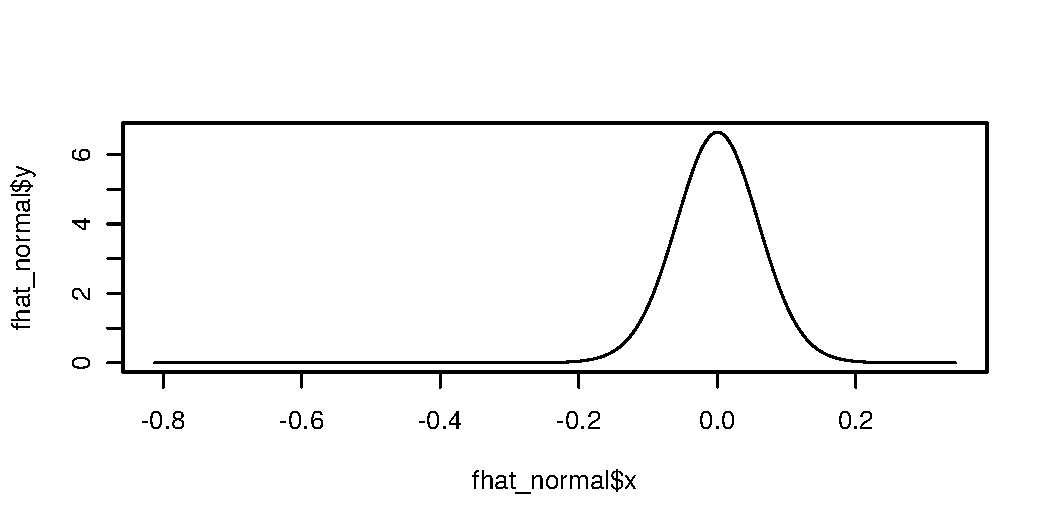
\includegraphics[width=\maxwidth]{figure/unnamed-chunk-17-1} 
\begin{kframe}\begin{alltt}
\hlstd{fhat_unif} \hlkwb{<-} \hlkwd{bkde}\hlstd{(x,} \hlkwc{kernel} \hlstd{=} \hlstr{"box"}\hlstd{,} \hlkwc{bandwidth} \hlstd{=} \hlnum{0.05}\hlstd{)}
\hlkwd{plot}\hlstd{(fhat_unif,} \hlkwc{type} \hlstd{=} \hlstr{"l"}\hlstd{)}
\end{alltt}
\end{kframe}
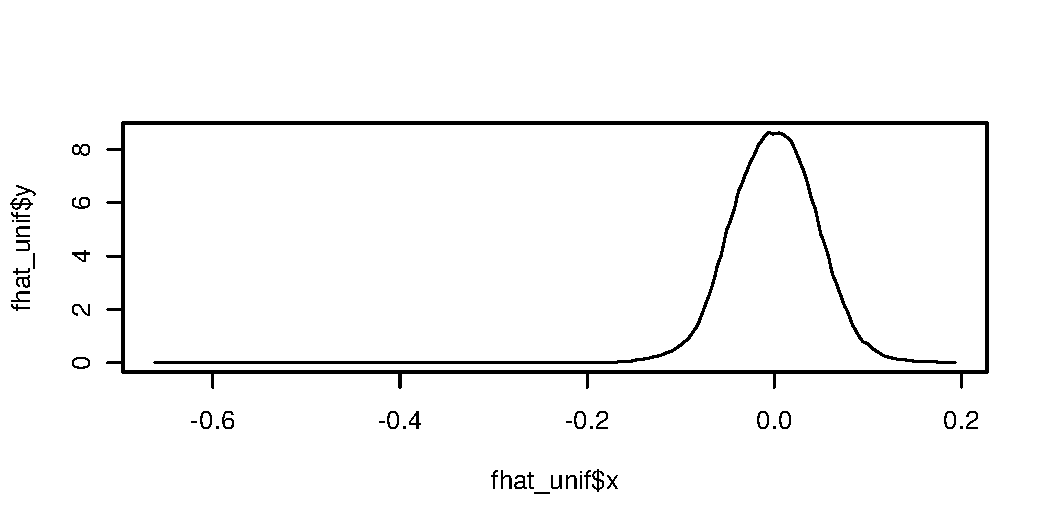
\includegraphics[width=\maxwidth]{figure/unnamed-chunk-17-2} 
\begin{kframe}\begin{alltt}
\hlstd{fhat_epanech} \hlkwb{<-} \hlkwd{bkde}\hlstd{(x,} \hlkwc{kernel} \hlstd{=} \hlstr{"epanech"}\hlstd{,} \hlkwc{bandwidth} \hlstd{=} \hlnum{0.05}\hlstd{)}
\hlkwd{plot}\hlstd{(fhat_epanech,} \hlkwc{type} \hlstd{=} \hlstr{"l"}\hlstd{)}
\end{alltt}
\end{kframe}
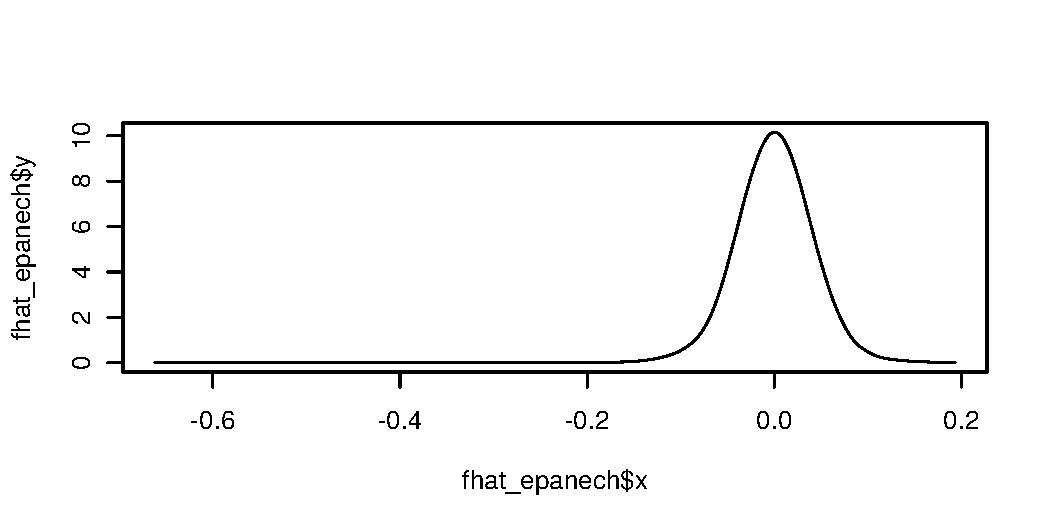
\includegraphics[width=\maxwidth]{figure/unnamed-chunk-17-3} 
\begin{kframe}\begin{alltt}
\hlstd{fhat_biweight} \hlkwb{<-} \hlkwd{bkde}\hlstd{(x,} \hlkwc{kernel} \hlstd{=} \hlstr{"biweight"}\hlstd{,} \hlkwc{bandwidth} \hlstd{=} \hlnum{0.05}\hlstd{)}
\hlkwd{plot}\hlstd{(fhat_biweight,} \hlkwc{type} \hlstd{=} \hlstr{"l"}\hlstd{)}
\end{alltt}
\end{kframe}
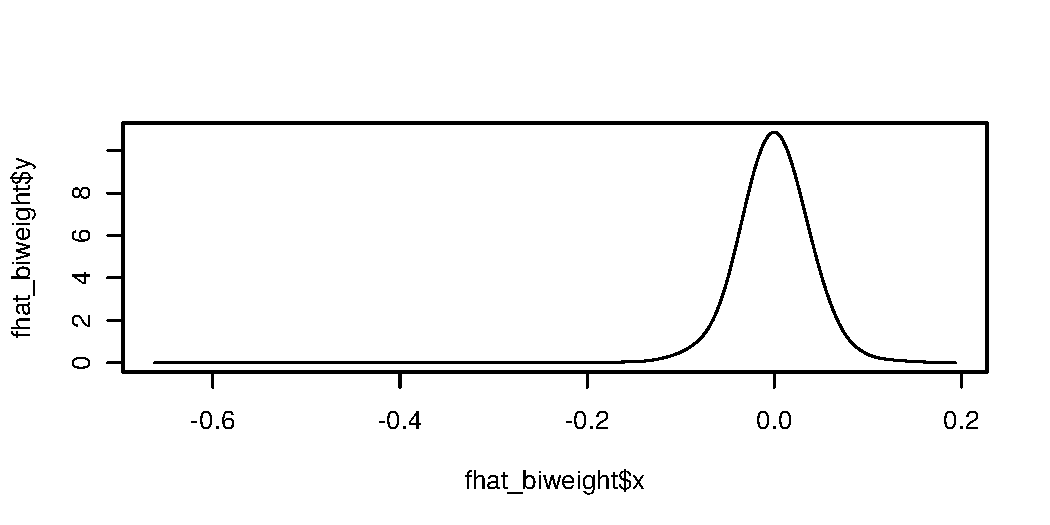
\includegraphics[width=\maxwidth]{figure/unnamed-chunk-17-4} 
\begin{kframe}\begin{alltt}
\hlstd{fhat_triweight} \hlkwb{<-} \hlkwd{bkde}\hlstd{(x,} \hlkwc{kernel} \hlstd{=} \hlstr{"triweight"}\hlstd{,} \hlkwc{bandwidth} \hlstd{=} \hlnum{0.05}\hlstd{)}
\hlkwd{plot}\hlstd{(fhat_triweight,} \hlkwc{type} \hlstd{=} \hlstr{"l"}\hlstd{)}
\end{alltt}
\end{kframe}
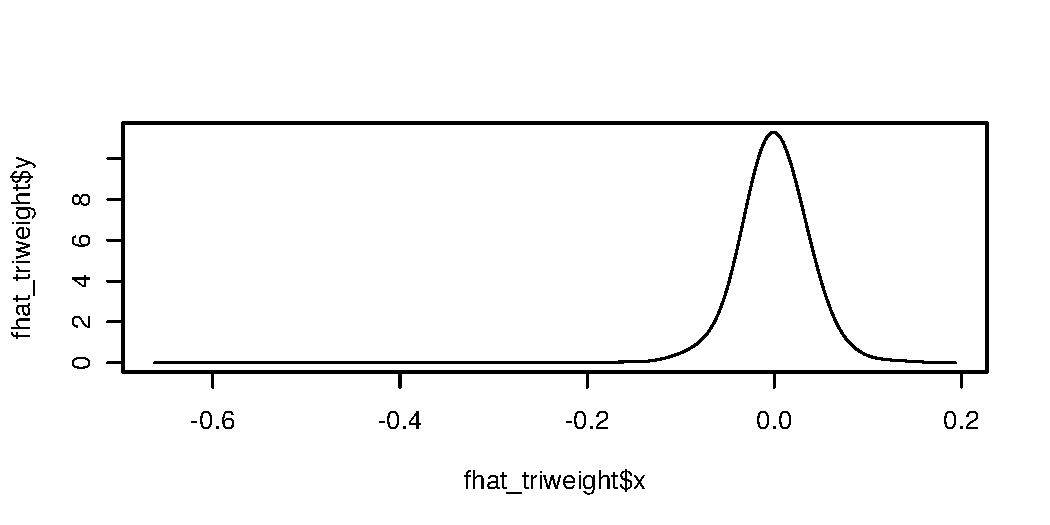
\includegraphics[width=\maxwidth]{figure/unnamed-chunk-17-5} 

\end{knitrout}

 \subsubsection{Efecto del ancho de banda en la estimación }

 \paragraph{Kernel uniforme}
\begin{knitrout}
\definecolor{shadecolor}{rgb}{1, 1, 1}\color{fgcolor}\begin{kframe}
\begin{alltt}
\hlstd{fhat} \hlkwb{<-} \hlkwd{bkde}\hlstd{(x,} \hlkwc{kernel} \hlstd{=} \hlstr{"box"}\hlstd{,} \hlkwc{bandwidth} \hlstd{=} \hlnum{0.001}\hlstd{)}
\end{alltt}


{\ttfamily\noindent\color{warningcolor}{\#\# Warning in bkde(x, kernel = "{}box"{}, bandwidth = 0.001): Binning grid too coarse for current (small) bandwidth: consider increasing 'gridsize'}}\begin{alltt}
\hlkwd{plot}\hlstd{(fhat,} \hlkwc{type} \hlstd{=} \hlstr{"l"}\hlstd{)}
\end{alltt}
\end{kframe}
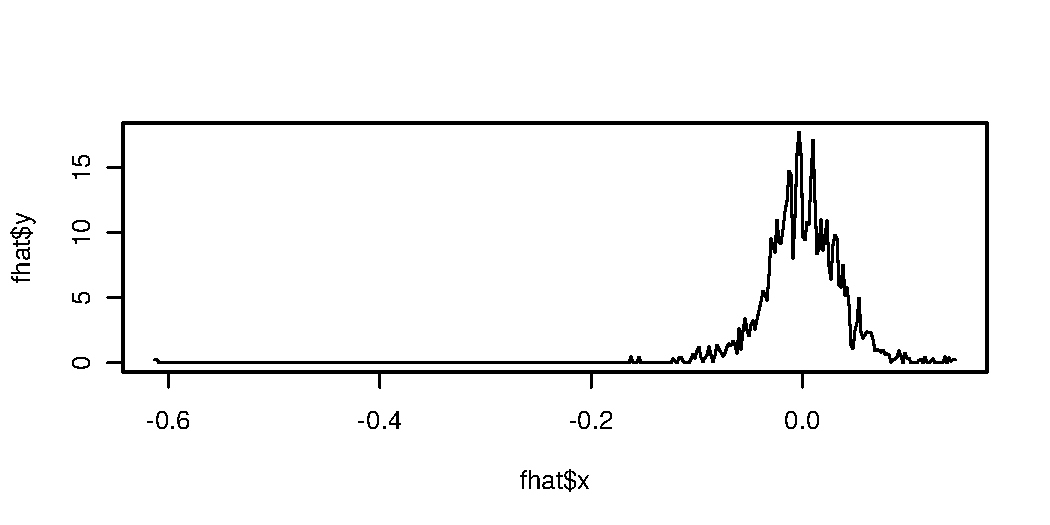
\includegraphics[width=\maxwidth]{figure/unnamed-chunk-18-1} 
\begin{kframe}\begin{alltt}
\hlstd{fhat} \hlkwb{<-} \hlkwd{bkde}\hlstd{(x,} \hlkwc{kernel} \hlstd{=} \hlstr{"box"}\hlstd{,} \hlkwc{bandwidth} \hlstd{=} \hlnum{0.5}\hlstd{)}
\hlkwd{plot}\hlstd{(fhat,} \hlkwc{type} \hlstd{=} \hlstr{"l"}\hlstd{)}
\end{alltt}
\end{kframe}
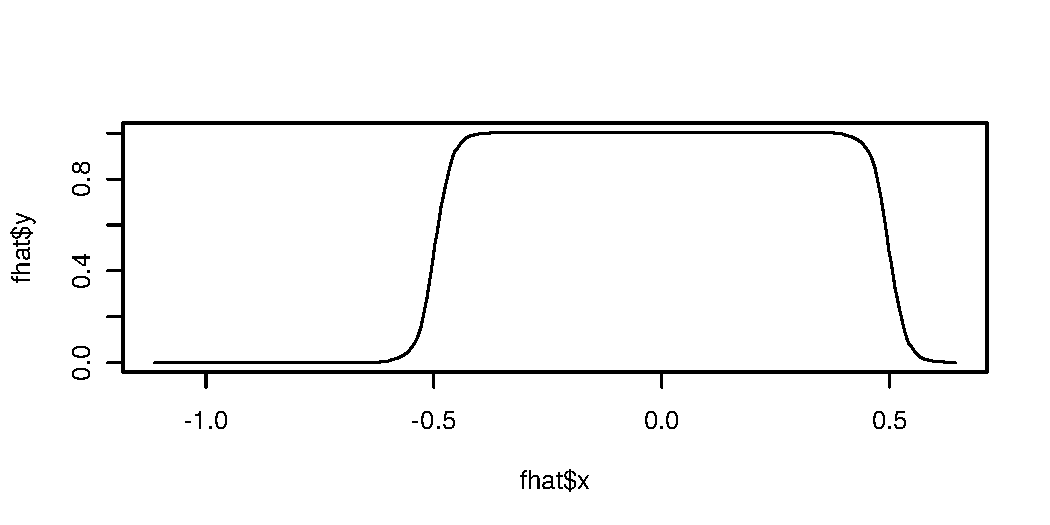
\includegraphics[width=\maxwidth]{figure/unnamed-chunk-18-2} 

\end{knitrout}


 \paragraph{Kernel Epanechnikov}

\begin{knitrout}
\definecolor{shadecolor}{rgb}{1, 1, 1}\color{fgcolor}\begin{kframe}
\begin{alltt}
\hlstd{fhat} \hlkwb{<-} \hlkwd{bkde}\hlstd{(x,} \hlkwc{kernel} \hlstd{=} \hlstr{"epa"}\hlstd{,} \hlkwc{bandwidth} \hlstd{=} \hlnum{0.001}\hlstd{)}
\end{alltt}


{\ttfamily\noindent\color{warningcolor}{\#\# Warning in bkde(x, kernel = "{}epa"{}, bandwidth = 0.001): Binning grid too coarse for current (small) bandwidth: consider increasing 'gridsize'}}\begin{alltt}
\hlkwd{plot}\hlstd{(fhat,} \hlkwc{type} \hlstd{=} \hlstr{"l"}\hlstd{)}
\end{alltt}
\end{kframe}
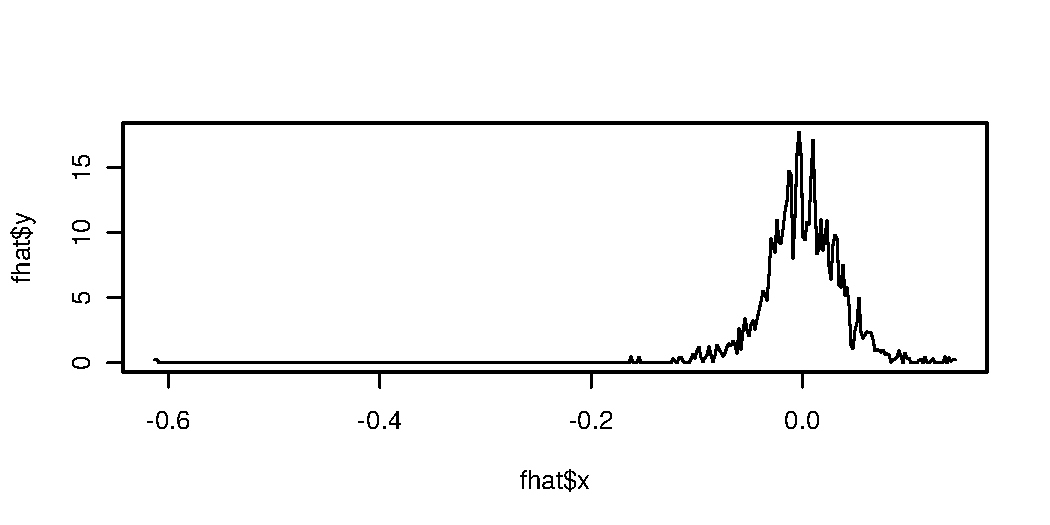
\includegraphics[width=\maxwidth]{figure/unnamed-chunk-19-1} 
\begin{kframe}\begin{alltt}
\hlstd{fhat} \hlkwb{<-} \hlkwd{bkde}\hlstd{(x,} \hlkwc{kernel} \hlstd{=} \hlstr{"epa"}\hlstd{,} \hlkwc{bandwidth} \hlstd{=} \hlnum{0.5}\hlstd{)}
\hlkwd{plot}\hlstd{(fhat,} \hlkwc{type} \hlstd{=} \hlstr{"l"}\hlstd{)}
\end{alltt}
\end{kframe}
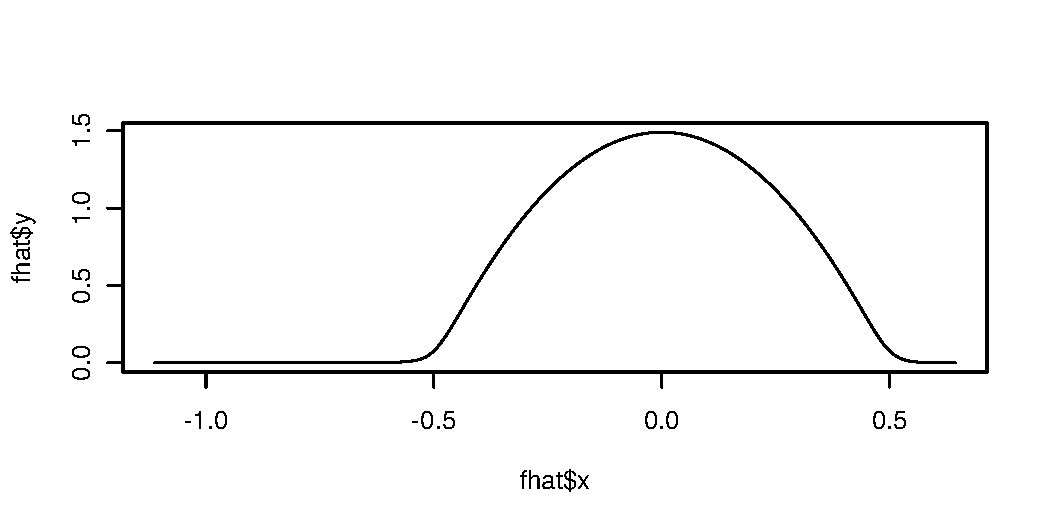
\includegraphics[width=\maxwidth]{figure/unnamed-chunk-19-2} 

\end{knitrout}


\begin{knitrout}
\definecolor{shadecolor}{rgb}{1, 1, 1}\color{fgcolor}\begin{kframe}
\begin{alltt}
\hlkwd{suppressMessages}\hlstd{(}\hlkwd{library}\hlstd{(tidyverse))}
\hlkwd{library}\hlstd{(gganimate)}

\hlstd{fani} \hlkwb{<-} \hlkwd{tibble}\hlstd{()}

\hlkwa{for} \hlstd{(b} \hlkwa{in} \hlkwd{seq}\hlstd{(}\hlnum{0.001}\hlstd{,} \hlnum{0.02}\hlstd{,} \hlkwc{length.out} \hlstd{=} \hlnum{40}\hlstd{)) \{}
 \hlstd{f} \hlkwb{<-} \hlkwd{bkde}\hlstd{(x,} \hlkwc{kernel} \hlstd{=} \hlstr{"epa"}\hlstd{,} \hlkwc{bandwidth} \hlstd{= b,} \hlkwc{gridsize} \hlstd{=} \hlkwd{length}\hlstd{(x))}
 \hlstd{fani} \hlkwb{<-} \hlstd{fani} \hlopt \hlkwd{bind_rows}\hlstd{(}\hlkwd{tibble}\hlstd{(}\hlkwc{xreal} \hlstd{=} \hlkwd{sort}\hlstd{(x),} \hlkwc{x} \hlstd{= f}\hlopt{$}\hlstd{x,} \hlkwc{y} \hlstd{= f}\hlopt{$}\hlstd{y,} \hlkwc{bw} \hlstd{= b))}
\hlstd{\}}

\hlkwd{ggplot}\hlstd{(}\hlkwc{data} \hlstd{= fani)} \hlopt{+}
 \hlkwd{geom_line}\hlstd{(}\hlkwd{aes}\hlstd{(x, y),} \hlkwc{color} \hlstd{=} \hlstr{"blue"}\hlstd{)} \hlopt{+}
 \hlkwd{labs}\hlstd{(}\hlkwc{title} \hlstd{=} \hlkwd{paste0}\hlstd{(}\hlstr{"Ancho de banda = \{closest_state\}"}\hlstd{))} \hlopt{+}
 \hlkwd{transition_states}\hlstd{(bw)} \hlopt{+}
 \hlkwd{view_follow}\hlstd{()} \hlopt{+}
 \hlkwd{theme_minimal}\hlstd{(}\hlkwc{base_size} \hlstd{=} \hlnum{20}\hlstd{)}

\hlkwd{anim_save}\hlstd{(}\hlstr{"manual_figure/bandwidth-animation.gif"}\hlstd{)}
\end{alltt}
\end{kframe}
\end{knitrout}


 \includemedia[
 label=bandwidth,
 width=0.6\linewidth,height=0.45\linewidth,
 addresource=manual_figure/bandwidth-animation.mp4,
 transparent,
 %transparent player background
 activate=pageopen,
 %show VPlayer's right-click menu
 flashvars={
 source=manual_figure/bandwidth-animation.mp4
 &loop=true
 % loop video
 }
 ]{}{VPlayer.swf}

 \begin{pregunta}{}{}

 \begin{enumerate}
 \item Construya una variable llamada `u` que sea una secuencia de -0.15 a 0.15 con un paso de 0.01
 \item Asigne `x` a los datos `stockrel` y calcule su media y varianza.
 \item Usando la función `dnorm` construya los valores de la distribución de los datos usando la media y varianza calculada anteriormente. Asigne a esta variable `f\_param`.
 \item Defina un ancho de banda `h` en 0.02
 \item Construya un histograma para estos datos con ancho de banda `h`. Llame a esta variable `f\_hist`
 \item Usando el paquete `KernSmooth` y la función `bkde`, construya una función que calcule el estimador no paramétrico con un núcleo Epanechivok para un ancho de banda  $h$.  Llame a esta variable `f\_epa`.
 \item Dibuje en el mismo gráfico la estimación paramétrica y no paramétrica.
 \end{enumerate}
 \end{pregunta}

 \begin{solucion}{}{}
\begin{knitrout}
\definecolor{shadecolor}{rgb}{1, 1, 1}\color{fgcolor}\begin{kframe}
\begin{alltt}
\hlstd{x} \hlkwb{<-} \hlkwd{read.csv}\hlstd{(}\hlstr{"data/stockres.txt"}\hlstd{)}
\hlstd{x} \hlkwb{<-} \hlkwd{unlist}\hlstd{(x)}
\hlcom{# Eliminar nombres de las columnas}
\hlkwd{names}\hlstd{(x)} \hlkwb{<-} \hlkwa{NULL}

\hlstd{u} \hlkwb{<-} \hlkwd{seq}\hlstd{(}\hlopt{-}\hlnum{0.15}\hlstd{,} \hlnum{0.15}\hlstd{,} \hlkwc{by} \hlstd{=} \hlnum{0.01}\hlstd{)}

\hlstd{mu} \hlkwb{<-} \hlkwd{mean}\hlstd{(x)}
\hlstd{sigma} \hlkwb{<-} \hlkwd{sd}\hlstd{(x)}

\hlstd{f_param} \hlkwb{<-} \hlkwd{dnorm}\hlstd{(u,} \hlkwc{mean} \hlstd{= mu,} \hlkwc{sd} \hlstd{= sigma)}

\hlstd{h} \hlkwb{<-} \hlnum{0.02}

\hlstd{n_bins} \hlkwb{<-} \hlkwd{floor}\hlstd{(}\hlkwd{diff}\hlstd{(}\hlkwd{range}\hlstd{(x))} \hlopt{/} \hlstd{h)}

\hlstd{f_hist} \hlkwb{<-} \hlkwd{hist}\hlstd{(x,} \hlkwc{breaks} \hlstd{= n_bins)}
\end{alltt}
\end{kframe}
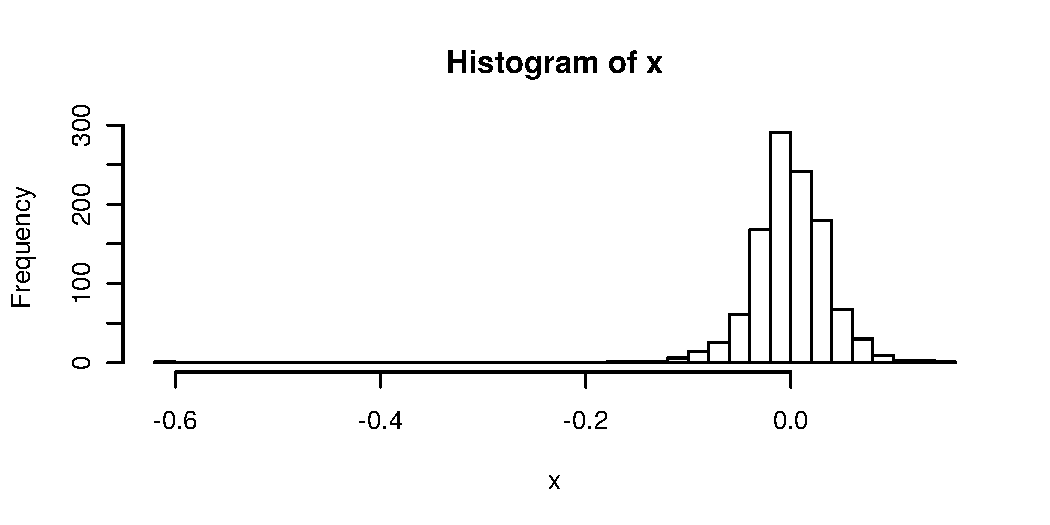
\includegraphics[width=\maxwidth]{figure/unnamed-chunk-21-1} 
\begin{kframe}\begin{alltt}
\hlstd{f_epa} \hlkwb{<-} \hlkwd{as.data.frame}\hlstd{(}\hlkwd{bkde}\hlstd{(x,} \hlkwc{kernel} \hlstd{=} \hlstr{"epa"}\hlstd{,} \hlkwc{bandwidth} \hlstd{= h))}

\hlstd{x_df} \hlkwb{<-} \hlkwd{data.frame}\hlstd{(x)}

\hlkwd{library}\hlstd{(ggplot2)}

\hlkwd{ggplot}\hlstd{(x_df,} \hlkwd{aes}\hlstd{(x))} \hlopt{+}
 \hlkwd{geom_histogram}\hlstd{(}
   \hlkwd{aes}\hlstd{(}\hlkwc{y} \hlstd{= ..density..),}
   \hlkwc{binwidth} \hlstd{=} \hlnum{0.02}\hlstd{,}
   \hlkwc{col} \hlstd{=} \hlstr{"black"}\hlstd{,}
   \hlkwc{fill} \hlstd{=} \hlstr{"white"}
 \hlstd{)} \hlopt{+}
 \hlkwd{stat_function}\hlstd{(}
   \hlkwc{fun} \hlstd{= dnorm,}
   \hlkwc{args} \hlstd{=} \hlkwd{list}\hlstd{(}\hlkwc{mean} \hlstd{= mu,} \hlkwc{sd} \hlstd{= sigma),}
   \hlkwc{color} \hlstd{=} \hlstr{"red"}
 \hlstd{)} \hlopt{+}
 \hlkwd{geom_line}\hlstd{(}\hlkwc{data} \hlstd{= f_epa,} \hlkwd{aes}\hlstd{(x, y),} \hlkwc{color} \hlstd{=} \hlstr{"blue"}\hlstd{)} \hlopt{+}
 \hlkwd{theme_minimal}\hlstd{(}\hlkwc{base_size} \hlstd{=} \hlnum{20}\hlstd{)}
\end{alltt}
\end{kframe}
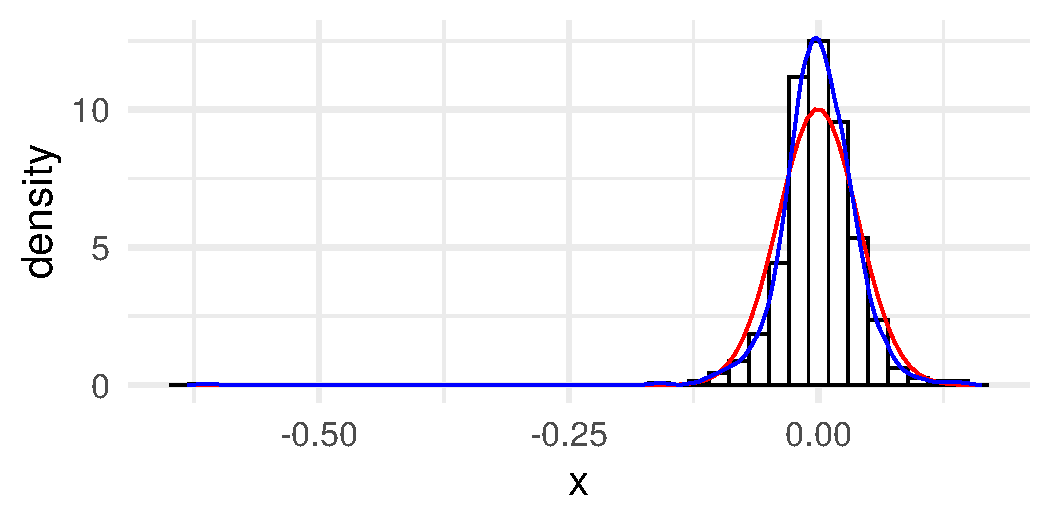
\includegraphics[width=\maxwidth]{figure/unnamed-chunk-21-2} 

\end{knitrout}


 \end{solucion}

 \subsubsection{Ancho de banda óptimo}

 Usemos la regla de la normal o también conocida como Silverman.
 \textbf{Primero recuerde que en este caso se asume que $f(x)$ sigue una distribución normal}. En este caso, lo que se obtiene es que

 \begin{align*}
 \Vert f^{\prime \prime} \Vert_2^2 & = \sigma ^{-5} \int \{\phi^{\prime \prime}\}^2 dx              \\
 & = \sigma ^{-5} \frac{3}{8\sqrt{\pi}} \approx 0.212 \sigma^{-5}
 \end{align*}

 donde $\phi$ es la densidad de una normal estándar.

 El estimador para $\sigma$ es

 \[
 s = \sqrt{\frac{1}{n-1} \sum_{i=1}^n (x_i - \bar{x})^2  }.
 \]

 Y usando el cálculo realizado anteriormente, se obtiene que

 \[
 h_{normal} = \left( \frac{4 s^5}{3n} \right)^{1/5} \approx 1.06 s n^{-1/5}.
 \]

 Un estimador más robusto es

 \[
 h_{normal} =  1.06 \min \left\{ s , \frac{IQR}{1.34} \right\} n^{-1/5}.
 \]

 ¿Por qué es $IQR / 1.34$?

\begin{knitrout}
\definecolor{shadecolor}{rgb}{1, 1, 1}\color{fgcolor}\begin{kframe}
\begin{alltt}
\hlstd{s} \hlkwb{<-} \hlkwd{sd}\hlstd{(x)}
\hlstd{n} \hlkwb{<-} \hlkwd{length}\hlstd{(x)}
\end{alltt}
\end{kframe}
\end{knitrout}


\begin{knitrout}
\definecolor{shadecolor}{rgb}{1, 1, 1}\color{fgcolor}\begin{kframe}
\begin{alltt}
\hlstd{h_normal} \hlkwb{<-} \hlnum{1.06} \hlopt{*} \hlstd{s} \hlopt{*} \hlstd{n}\hlopt{^}\hlstd{(}\hlopt{-}\hlnum{1} \hlopt{/} \hlnum{5}\hlstd{)}

\hlstd{h} \hlkwb{<-} \hlstd{h_normal}

\hlstd{n_bins} \hlkwb{<-} \hlkwd{floor}\hlstd{(}\hlkwd{diff}\hlstd{(}\hlkwd{range}\hlstd{(x))} \hlopt{/} \hlstd{h)}
\hlstd{f_hist} \hlkwb{<-} \hlkwd{hist}\hlstd{(x,} \hlkwc{breaks} \hlstd{= n_bins,} \hlkwc{plot} \hlstd{=} \hlnum{FALSE}\hlstd{)}
\hlstd{f_epa} \hlkwb{<-} \hlkwd{as.data.frame}\hlstd{(}\hlkwd{bkde}\hlstd{(x,} \hlkwc{kernel} \hlstd{=} \hlstr{"epa"}\hlstd{,} \hlkwc{bandwidth} \hlstd{= h))}

\hlkwd{ggplot}\hlstd{(x_df,} \hlkwd{aes}\hlstd{(x))} \hlopt{+}
 \hlkwd{geom_histogram}\hlstd{(}
   \hlkwd{aes}\hlstd{(}\hlkwc{y} \hlstd{= ..density..),}
   \hlkwc{binwidth} \hlstd{= h,}
   \hlkwc{col} \hlstd{=} \hlstr{"black"}\hlstd{,}
   \hlkwc{fill} \hlstd{=} \hlstr{"white"}
 \hlstd{)} \hlopt{+}
 \hlkwd{stat_function}\hlstd{(}
   \hlkwc{fun} \hlstd{= dnorm,}
   \hlkwc{args} \hlstd{=} \hlkwd{list}\hlstd{(}\hlkwc{mean} \hlstd{= mu,} \hlkwc{sd} \hlstd{= sigma),}
   \hlkwc{color} \hlstd{=} \hlstr{"red"}
 \hlstd{)} \hlopt{+}
 \hlkwd{geom_line}\hlstd{(}\hlkwc{data} \hlstd{= f_epa,} \hlkwd{aes}\hlstd{(x, y),} \hlkwc{color} \hlstd{=} \hlstr{"blue"}\hlstd{)} \hlopt{+}
 \hlkwd{theme_minimal}\hlstd{(}\hlkwc{base_size} \hlstd{=} \hlnum{20}\hlstd{)}
\end{alltt}
\end{kframe}
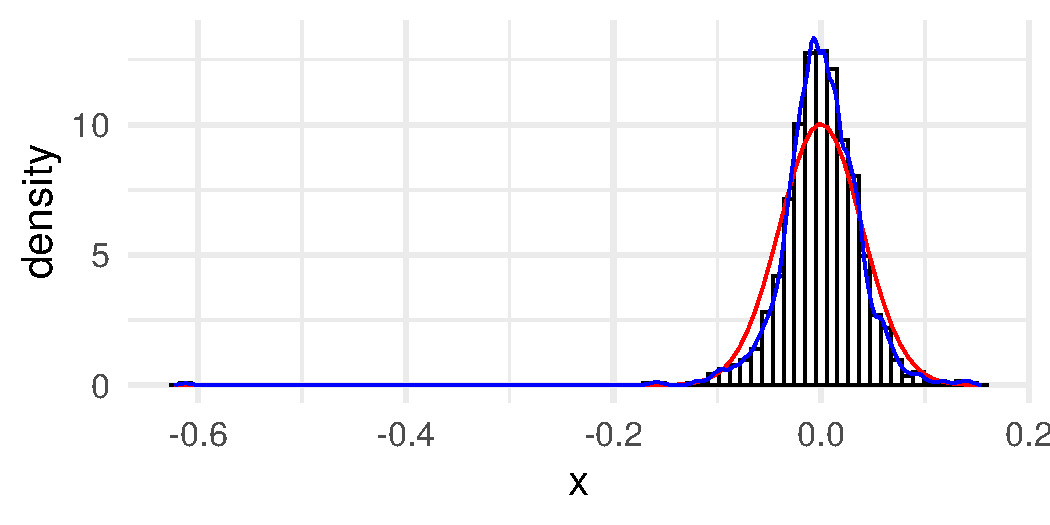
\includegraphics[width=\maxwidth]{figure/unnamed-chunk-23-1} 

\end{knitrout}


\begin{knitrout}
\definecolor{shadecolor}{rgb}{1, 1, 1}\color{fgcolor}\begin{kframe}
\begin{alltt}
\hlstd{h_iqr} \hlkwb{<-} \hlnum{1.06} \hlopt{*} \hlkwd{min}\hlstd{(s,} \hlkwd{IQR}\hlstd{(x)} \hlopt{/} \hlnum{1.34}\hlstd{)} \hlopt{*} \hlstd{n}\hlopt{^}\hlstd{(}\hlopt{-}\hlnum{1} \hlopt{/} \hlnum{5}\hlstd{)}

\hlstd{h} \hlkwb{<-} \hlstd{h_iqr}

\hlstd{n_bins} \hlkwb{<-} \hlkwd{floor}\hlstd{(}\hlkwd{diff}\hlstd{(}\hlkwd{range}\hlstd{(x))} \hlopt{/} \hlstd{h)}
\hlstd{f_hist} \hlkwb{<-} \hlkwd{hist}\hlstd{(x,} \hlkwc{breaks} \hlstd{= n_bins,} \hlkwc{plot} \hlstd{=} \hlnum{FALSE}\hlstd{)}
\hlstd{f_epa} \hlkwb{<-} \hlkwd{as.data.frame}\hlstd{(}\hlkwd{bkde}\hlstd{(x,} \hlkwc{kernel} \hlstd{=} \hlstr{"epa"}\hlstd{,} \hlkwc{bandwidth} \hlstd{= h))}

\hlkwd{ggplot}\hlstd{(x_df,} \hlkwd{aes}\hlstd{(x))} \hlopt{+}
 \hlkwd{geom_histogram}\hlstd{(}
   \hlkwd{aes}\hlstd{(}\hlkwc{y} \hlstd{= ..density..),}
   \hlkwc{binwidth} \hlstd{= h,}
   \hlkwc{col} \hlstd{=} \hlstr{"black"}\hlstd{,}
   \hlkwc{fill} \hlstd{=} \hlstr{"white"}
 \hlstd{)} \hlopt{+}
 \hlkwd{stat_function}\hlstd{(}
   \hlkwc{fun} \hlstd{= dnorm,}
   \hlkwc{args} \hlstd{=} \hlkwd{list}\hlstd{(}\hlkwc{mean} \hlstd{= mu,} \hlkwc{sd} \hlstd{= sigma),}
   \hlkwc{color} \hlstd{=} \hlstr{"red"}
 \hlstd{)} \hlopt{+}
 \hlkwd{geom_line}\hlstd{(}\hlkwc{data} \hlstd{= f_epa,} \hlkwd{aes}\hlstd{(x, y),} \hlkwc{color} \hlstd{=} \hlstr{"blue"}\hlstd{)} \hlopt{+}
 \hlkwd{theme_minimal}\hlstd{(}\hlkwc{base_size} \hlstd{=} \hlnum{20}\hlstd{)}
\end{alltt}
\end{kframe}
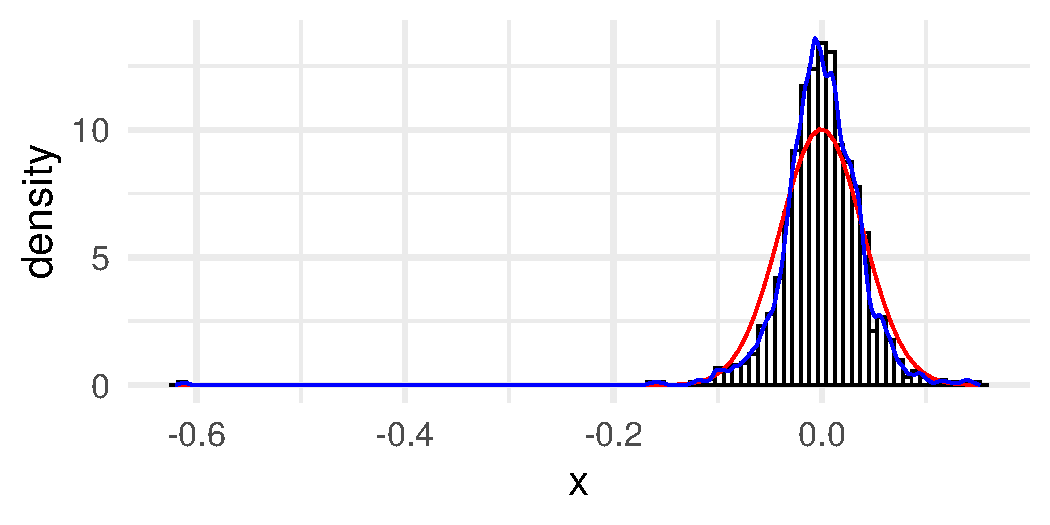
\includegraphics[width=\maxwidth]{figure/unnamed-chunk-24-1} 

\end{knitrout}


 Una librería más especializada es \texttt{np} (non-parametric).

\begin{knitrout}
\definecolor{shadecolor}{rgb}{1, 1, 1}\color{fgcolor}\begin{kframe}
\begin{alltt}
\hlkwd{library}\hlstd{(np)}

\hlstd{x.eval} \hlkwb{<-} \hlkwd{seq}\hlstd{(}\hlopt{-}\hlnum{0.2}\hlstd{,} \hlnum{0.2}\hlstd{,} \hlkwc{length.out} \hlstd{=} \hlnum{200}\hlstd{)}

\hlstd{h_normal_np} \hlkwb{<-} \hlkwd{npudensbw}\hlstd{(}\hlkwc{dat} \hlstd{= x,} \hlkwc{bwmethod} \hlstd{=} \hlstr{"normal-reference"}\hlstd{)}

\hlstd{dens.ksum} \hlkwb{<-} \hlkwd{npksum}\hlstd{(}
 \hlkwc{txdat} \hlstd{= x,}
 \hlkwc{exdat} \hlstd{= x.eval,}
 \hlkwc{bws} \hlstd{= h_normal_np}\hlopt{$}\hlstd{bw}
\hlstd{)}\hlopt{$}\hlstd{ksum} \hlopt{/} \hlstd{(n} \hlopt{*} \hlstd{h_normal_np}\hlopt{$}\hlstd{bw[}\hlnum{1}\hlstd{])}

\hlstd{dens.ksum.df} \hlkwb{<-} \hlkwd{data.frame}\hlstd{(}\hlkwc{x} \hlstd{= x.eval,} \hlkwc{y} \hlstd{= dens.ksum)}

\hlkwd{ggplot}\hlstd{(x_df,} \hlkwd{aes}\hlstd{(x))} \hlopt{+}
 \hlkwd{geom_histogram}\hlstd{(}
   \hlkwd{aes}\hlstd{(}\hlkwc{y} \hlstd{= ..density..),}
   \hlkwc{binwidth} \hlstd{= h_normal_np}\hlopt{$}\hlstd{bw,}
   \hlkwc{col} \hlstd{=} \hlstr{"black"}\hlstd{,}
   \hlkwc{fill} \hlstd{=} \hlstr{"white"}
 \hlstd{)} \hlopt{+}
 \hlkwd{stat_function}\hlstd{(}
   \hlkwc{fun} \hlstd{= dnorm,}
   \hlkwc{args} \hlstd{=} \hlkwd{list}\hlstd{(}\hlkwc{mean} \hlstd{= mu,} \hlkwc{sd} \hlstd{= sigma),}
   \hlkwc{color} \hlstd{=} \hlstr{"red"}
 \hlstd{)} \hlopt{+}
 \hlkwd{geom_line}\hlstd{(}\hlkwc{data} \hlstd{= dens.ksum.df,} \hlkwd{aes}\hlstd{(x, y),} \hlkwc{color} \hlstd{=} \hlstr{"blue"}\hlstd{)} \hlopt{+}
 \hlkwd{theme_minimal}\hlstd{(}\hlkwc{base_size} \hlstd{=} \hlnum{20}\hlstd{)}
\end{alltt}
\end{kframe}
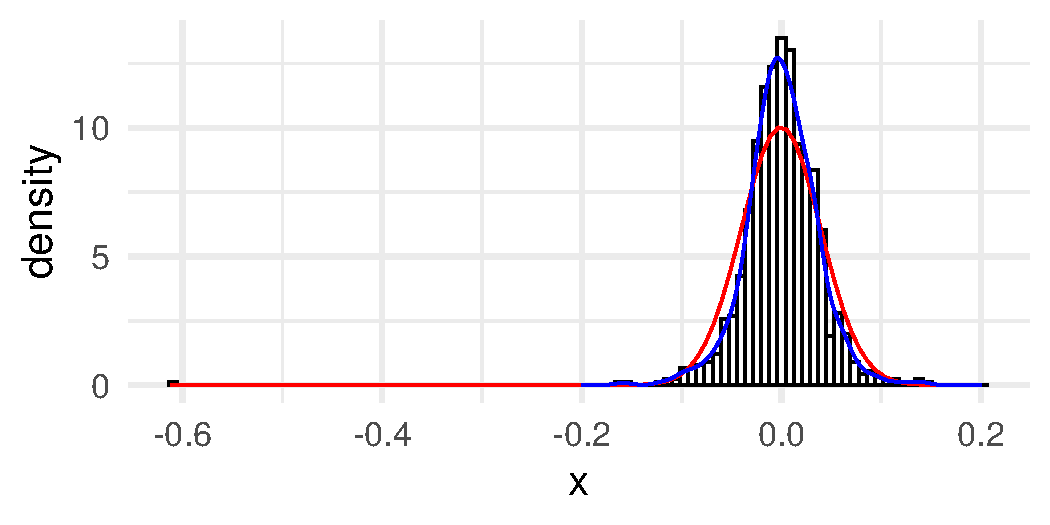
\includegraphics[width=\maxwidth]{figure/unnamed-chunk-25-1} 

\end{knitrout}


 \subsubsection{Validación cruzada}

 La forma que vimos en clase es la de validación cruzada por mínimos
 cuadrados``least-square cross validation'' la cual se puede ejecutar
 con este comando.

\begin{knitrout}
\definecolor{shadecolor}{rgb}{1, 1, 1}\color{fgcolor}\begin{kframe}
\begin{alltt}
\hlstd{h_cv_np_ls} \hlkwb{<-} \hlkwd{npudensbw}\hlstd{(}
 \hlkwc{dat} \hlstd{= x,}
 \hlkwc{bwmethod} \hlstd{=} \hlstr{"cv.ls"}\hlstd{,}
 \hlkwc{ckertype} \hlstd{=} \hlstr{"epa"}\hlstd{,}
 \hlkwc{ckerorder} \hlstd{=} \hlnum{2}
\hlstd{)}
\end{alltt}
\begin{verbatim}
## 
Multistart 1 of 1 |
Multistart 1 of 1 |
Multistart 1 of 1 |
Multistart 1 of 1 /
Multistart 1 of 1 |
Multistart 1 of 1 |
                   
\end{verbatim}
\begin{alltt}
\hlstd{dens.np} \hlkwb{<-} \hlkwd{npudens}\hlstd{(h_cv_np_ls)}

\hlkwd{plot}\hlstd{(dens.np,} \hlkwc{type} \hlstd{=} \hlstr{"b"}\hlstd{)}
\end{alltt}
\end{kframe}
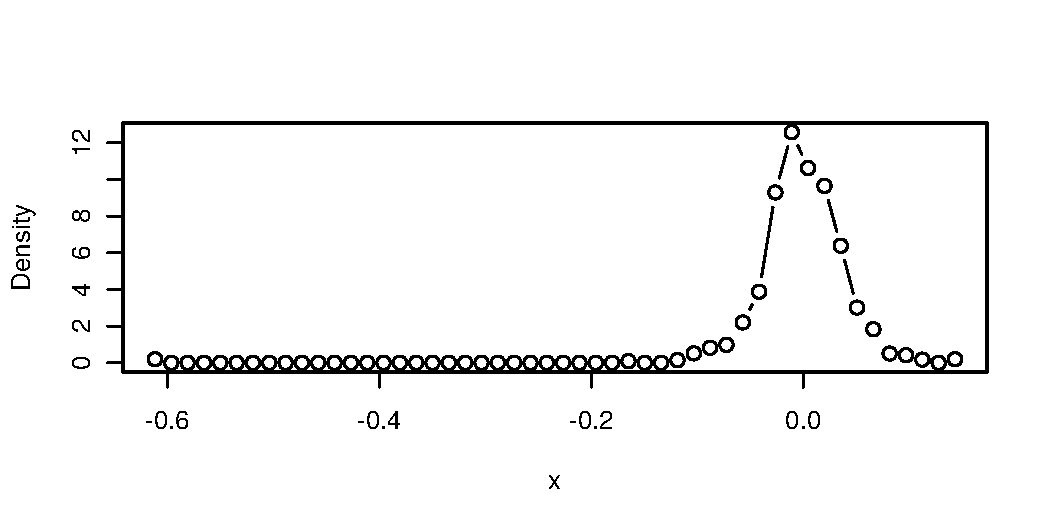
\includegraphics[width=\maxwidth]{figure/unnamed-chunk-26-1} 

\end{knitrout}


\begin{knitrout}
\definecolor{shadecolor}{rgb}{1, 1, 1}\color{fgcolor}\begin{kframe}
\begin{alltt}
\hlstd{dens.np.df} \hlkwb{<-} \hlkwd{data.frame}\hlstd{(}
 \hlkwc{x} \hlstd{= dens.np}\hlopt{$}\hlstd{eval[,} \hlnum{1}\hlstd{],}
 \hlkwc{y} \hlstd{= dens.np}\hlopt{$}\hlstd{dens}
\hlstd{)}

\hlkwd{ggplot}\hlstd{(x_df,} \hlkwd{aes}\hlstd{(x))} \hlopt{+}
 \hlkwd{geom_histogram}\hlstd{(}
   \hlkwd{aes}\hlstd{(}\hlkwc{y} \hlstd{= ..density..),}
   \hlkwc{binwidth} \hlstd{= h_cv_np_ls}\hlopt{$}\hlstd{bw,}
   \hlkwc{col} \hlstd{=} \hlstr{"black"}\hlstd{,}
   \hlkwc{fill} \hlstd{=} \hlstr{"white"}
 \hlstd{)} \hlopt{+}
 \hlkwd{stat_function}\hlstd{(}
   \hlkwc{fun} \hlstd{= dnorm,}
   \hlkwc{args} \hlstd{=} \hlkwd{list}\hlstd{(}\hlkwc{mean} \hlstd{= mu,} \hlkwc{sd} \hlstd{= sigma),}
   \hlkwc{color} \hlstd{=} \hlstr{"red"}
 \hlstd{)} \hlopt{+}
 \hlkwd{geom_line}\hlstd{(}\hlkwc{data} \hlstd{= dens.np.df,} \hlkwd{aes}\hlstd{(x, y),} \hlkwc{color} \hlstd{=} \hlstr{"blue"}\hlstd{)} \hlopt{+}
 \hlkwd{theme_minimal}\hlstd{(}\hlkwc{base_size} \hlstd{=} \hlnum{20}\hlstd{)}
\end{alltt}
\end{kframe}
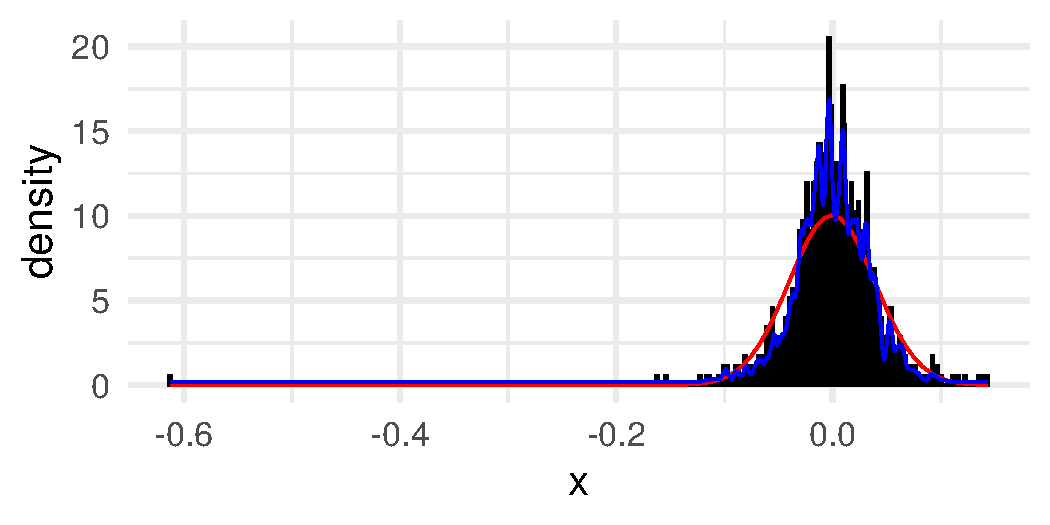
\includegraphics[width=\maxwidth]{figure/unnamed-chunk-27-1} 

\end{knitrout}


 \subsubsection{Temas adicionales}

 \paragraph{Reducción del sesgo}
 Como lo mencionamos en el texto, una forma de mejorar el sesgo en la estimación es suponer que la función de densidad es más veces diferenciable.

 Esto se logra asumiendo que el Kernel es más veces diferenciable.

\begin{knitrout}
\definecolor{shadecolor}{rgb}{1, 1, 1}\color{fgcolor}\begin{kframe}
\begin{alltt}
\hlstd{h_cv_np_ls} \hlkwb{<-} \hlkwd{npudensbw}\hlstd{(}
 \hlkwc{dat} \hlstd{= x,}
 \hlkwc{bwmethod} \hlstd{=} \hlstr{"cv.ls"}\hlstd{,}
 \hlkwc{ckertype} \hlstd{=} \hlstr{"epa"}\hlstd{,}
 \hlkwc{ckerorder} \hlstd{=} \hlnum{4}
\hlstd{)}
\end{alltt}
\begin{verbatim}
## 
Multistart 1 of 1 |
Multistart 1 of 1 |
Multistart 1 of 1 |
Multistart 1 of 1 /
Multistart 1 of 1 |
Multistart 1 of 1 |
                   
\end{verbatim}
\begin{alltt}
\hlstd{dens.np} \hlkwb{<-} \hlkwd{npudens}\hlstd{(h_cv_np_ls)}

\hlkwd{plot}\hlstd{(dens.np,} \hlkwc{type} \hlstd{=} \hlstr{"b"}\hlstd{,} \hlkwc{lwd} \hlstd{=} \hlnum{2}\hlstd{)}
\end{alltt}
\end{kframe}
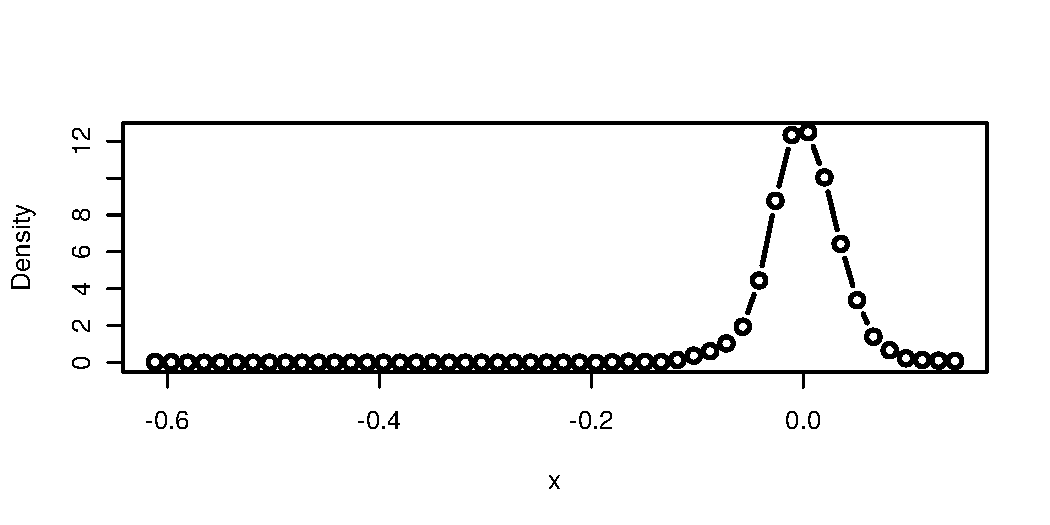
\includegraphics[width=\maxwidth]{figure/unnamed-chunk-28-1} 

\end{knitrout}


\begin{knitrout}
\definecolor{shadecolor}{rgb}{1, 1, 1}\color{fgcolor}\begin{kframe}
\begin{alltt}
\hlstd{dens.np.df} \hlkwb{<-} \hlkwd{data.frame}\hlstd{(}\hlkwc{x} \hlstd{= dens.np}\hlopt{$}\hlstd{eval[,} \hlnum{1}\hlstd{],} \hlkwc{y} \hlstd{= dens.np}\hlopt{$}\hlstd{dens)}

\hlkwd{ggplot}\hlstd{(x_df,} \hlkwd{aes}\hlstd{(x))} \hlopt{+}
 \hlkwd{geom_histogram}\hlstd{(}
   \hlkwd{aes}\hlstd{(}\hlkwc{y} \hlstd{= ..density..),}
   \hlkwc{binwidth} \hlstd{= h_cv_np_ls}\hlopt{$}\hlstd{bw,}
   \hlkwc{col} \hlstd{=} \hlstr{"black"}\hlstd{,}
   \hlkwc{fill} \hlstd{=} \hlstr{"white"}
 \hlstd{)} \hlopt{+}
 \hlkwd{stat_function}\hlstd{(}
   \hlkwc{fun} \hlstd{= dnorm,}
   \hlkwc{args} \hlstd{=} \hlkwd{list}\hlstd{(}\hlkwc{mean} \hlstd{= mu,} \hlkwc{sd} \hlstd{= sigma),}
   \hlkwc{color} \hlstd{=} \hlstr{"red"}
 \hlstd{)} \hlopt{+}
 \hlkwd{geom_line}\hlstd{(}\hlkwc{data} \hlstd{= dens.np.df,} \hlkwd{aes}\hlstd{(x, y),} \hlkwc{color} \hlstd{=} \hlstr{"blue"}\hlstd{)} \hlopt{+}
 \hlkwd{theme_minimal}\hlstd{(}\hlkwc{base_size} \hlstd{=} \hlnum{20}\hlstd{)}
\end{alltt}
\end{kframe}
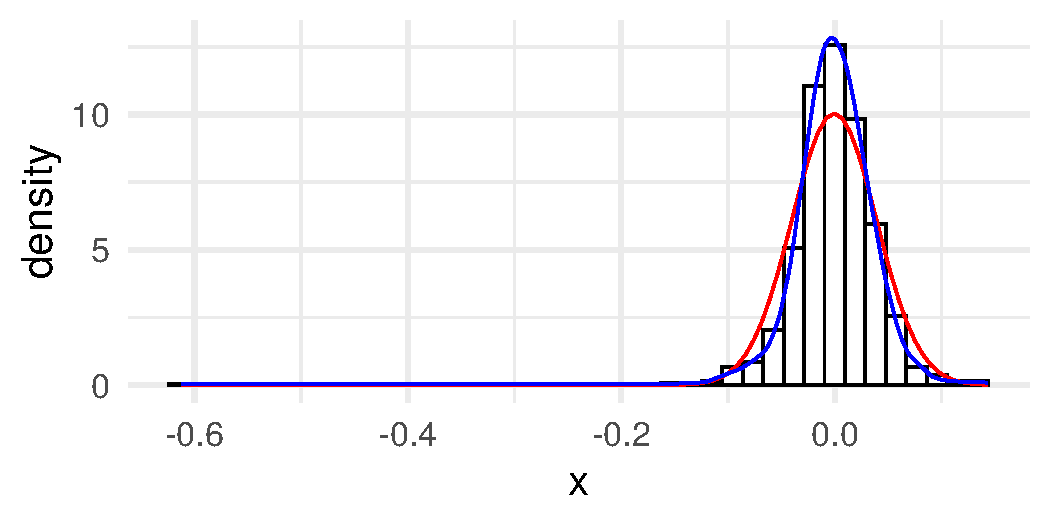
\includegraphics[width=\maxwidth]{figure/unnamed-chunk-29-1} 

\end{knitrout}


 \paragraph{Otra forma de estimar el ancho de banda} Otra forma de estimar ancho de bandas óptimos es usando máxima verosimilitud. Les dejo de tarea revisar la sección 1.1 del artículo de~\textcite{Hall1987} para entender su estructura.

\begin{knitrout}
\definecolor{shadecolor}{rgb}{1, 1, 1}\color{fgcolor}\begin{kframe}
\begin{alltt}
\hlstd{h_cv_np_ml} \hlkwb{<-} \hlkwd{npudensbw}\hlstd{(}
 \hlkwc{dat} \hlstd{= x,}
 \hlkwc{bwmethod} \hlstd{=} \hlstr{"cv.ml"}\hlstd{,}
 \hlkwc{ckertype} \hlstd{=} \hlstr{"epanechnikov"}
\hlstd{)}
\end{alltt}
\begin{verbatim}
## 
Multistart 1 of 1 |
Multistart 1 of 1 |
Multistart 1 of 1 |
Multistart 1 of 1 /
Multistart 1 of 1 |
Multistart 1 of 1 |
                   
\end{verbatim}
\begin{alltt}
\hlstd{dens.np} \hlkwb{<-} \hlkwd{npudens}\hlstd{(h_cv_np_ml)}

\hlkwd{plot}\hlstd{(dens.np,} \hlkwc{type} \hlstd{=} \hlstr{"b"}\hlstd{)}
\end{alltt}
\end{kframe}
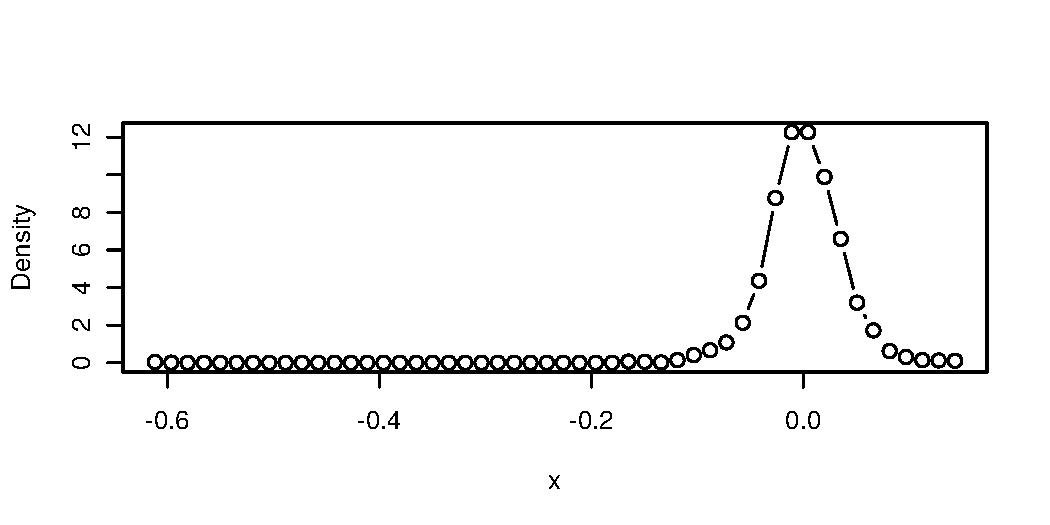
\includegraphics[width=\maxwidth]{figure/unnamed-chunk-30-1} 

\end{knitrout}


\begin{knitrout}
\definecolor{shadecolor}{rgb}{1, 1, 1}\color{fgcolor}\begin{kframe}
\begin{alltt}
\hlstd{dens.np.df} \hlkwb{<-} \hlkwd{data.frame}\hlstd{(}\hlkwc{x} \hlstd{= dens.np}\hlopt{$}\hlstd{eval[,} \hlnum{1}\hlstd{],} \hlkwc{y} \hlstd{= dens.np}\hlopt{$}\hlstd{dens)}

\hlkwd{ggplot}\hlstd{(x_df,} \hlkwd{aes}\hlstd{(x))} \hlopt{+}
 \hlkwd{geom_histogram}\hlstd{(}
   \hlkwd{aes}\hlstd{(}\hlkwc{y} \hlstd{= ..density..),}
   \hlkwc{binwidth} \hlstd{= h_cv_np_ml}\hlopt{$}\hlstd{bw,}
   \hlkwc{col} \hlstd{=} \hlstr{"black"}\hlstd{,}
   \hlkwc{fill} \hlstd{=} \hlstr{"white"}
 \hlstd{)} \hlopt{+}
 \hlkwd{stat_function}\hlstd{(}
   \hlkwc{fun} \hlstd{= dnorm,}
   \hlkwc{args} \hlstd{=} \hlkwd{list}\hlstd{(}\hlkwc{mean} \hlstd{= mu,} \hlkwc{sd} \hlstd{= sigma),}
   \hlkwc{color} \hlstd{=} \hlstr{"red"}
 \hlstd{)} \hlopt{+}
 \hlkwd{geom_line}\hlstd{(}\hlkwc{data} \hlstd{= dens.np.df,} \hlkwd{aes}\hlstd{(x, y),} \hlkwc{color} \hlstd{=} \hlstr{"blue"}\hlstd{)} \hlopt{+}
 \hlkwd{theme_minimal}\hlstd{(}\hlkwc{base_size} \hlstd{=} \hlnum{20}\hlstd{)}
\end{alltt}
\end{kframe}
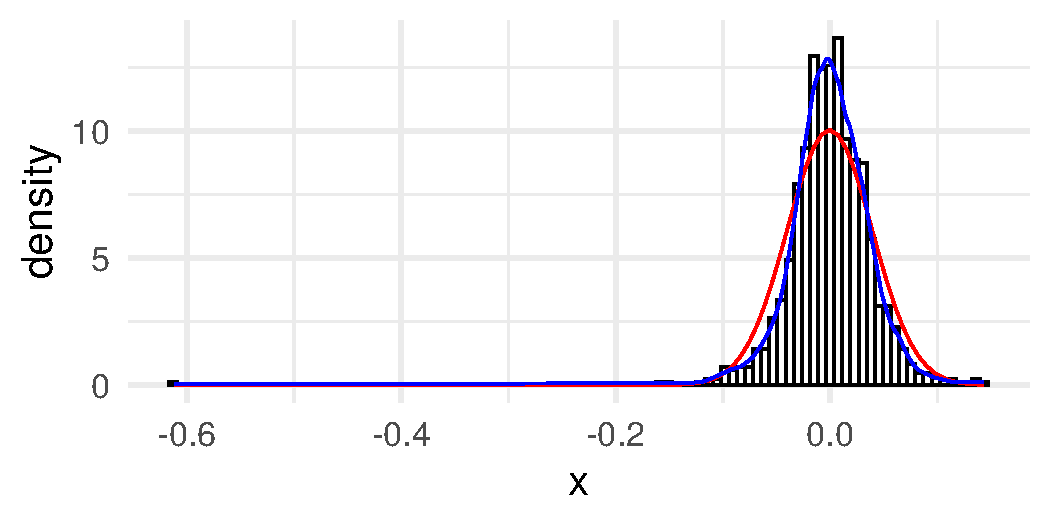
\includegraphics[width=\maxwidth]{figure/unnamed-chunk-31-1} 

\end{knitrout}


\begin{knitrout}
\definecolor{shadecolor}{rgb}{1, 1, 1}\color{fgcolor}\begin{kframe}
\begin{alltt}
\hlstd{h_cv_np_ml} \hlkwb{<-} \hlkwd{npudensbw}\hlstd{(}
 \hlkwc{dat} \hlstd{= x,}
 \hlkwc{bwmethod} \hlstd{=} \hlstr{"cv.ml"}\hlstd{,}
 \hlkwc{ckertype} \hlstd{=} \hlstr{"epanechnikov"}\hlstd{,}
 \hlkwc{ckerorder} \hlstd{=} \hlnum{4}
\hlstd{)}
\end{alltt}
\begin{verbatim}
## 
Multistart 1 of 1 |
Multistart 1 of 1 |
Multistart 1 of 1 |
Multistart 1 of 1 /
Multistart 1 of 1 |
Multistart 1 of 1 |
                   
\end{verbatim}
\begin{alltt}
\hlstd{dens.np} \hlkwb{<-} \hlkwd{npudens}\hlstd{(h_cv_np_ml)}

\hlkwd{plot}\hlstd{(dens.np,} \hlkwc{type} \hlstd{=} \hlstr{"b"}\hlstd{)}
\end{alltt}
\end{kframe}
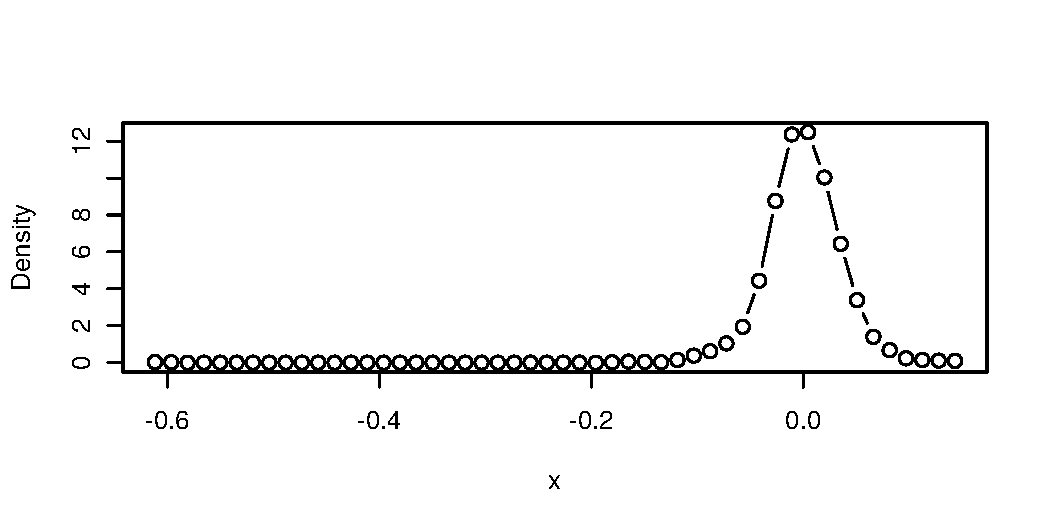
\includegraphics[width=\maxwidth]{figure/unnamed-chunk-32-1} 

\end{knitrout}


\begin{knitrout}
\definecolor{shadecolor}{rgb}{1, 1, 1}\color{fgcolor}\begin{kframe}
\begin{alltt}
\hlstd{dens.np.df} \hlkwb{<-} \hlkwd{data.frame}\hlstd{(}\hlkwc{x} \hlstd{= dens.np}\hlopt{$}\hlstd{eval[,} \hlnum{1}\hlstd{],} \hlkwc{y} \hlstd{= dens.np}\hlopt{$}\hlstd{dens)}

\hlkwd{ggplot}\hlstd{(x_df,} \hlkwd{aes}\hlstd{(x))} \hlopt{+}
 \hlkwd{geom_histogram}\hlstd{(}
   \hlkwd{aes}\hlstd{(}\hlkwc{y} \hlstd{= ..density..),}
   \hlkwc{binwidth} \hlstd{= h_cv_np_ml}\hlopt{$}\hlstd{bw,}
   \hlkwc{col} \hlstd{=} \hlstr{"black"}\hlstd{,}
   \hlkwc{fill} \hlstd{=} \hlstr{"white"}
 \hlstd{)} \hlopt{+}
 \hlkwd{stat_function}\hlstd{(}
   \hlkwc{fun} \hlstd{= dnorm,}
   \hlkwc{args} \hlstd{=} \hlkwd{list}\hlstd{(}\hlkwc{mean} \hlstd{= mu,} \hlkwc{sd} \hlstd{= sigma),}
   \hlkwc{color} \hlstd{=} \hlstr{"red"}
 \hlstd{)} \hlopt{+}
 \hlkwd{geom_line}\hlstd{(}\hlkwc{data} \hlstd{= dens.np.df,} \hlkwd{aes}\hlstd{(x, y),} \hlkwc{color} \hlstd{=} \hlstr{"blue"}\hlstd{)} \hlopt{+}
 \hlkwd{theme_minimal}\hlstd{(}\hlkwc{base_size} \hlstd{=} \hlnum{20}\hlstd{)}
\end{alltt}
\end{kframe}
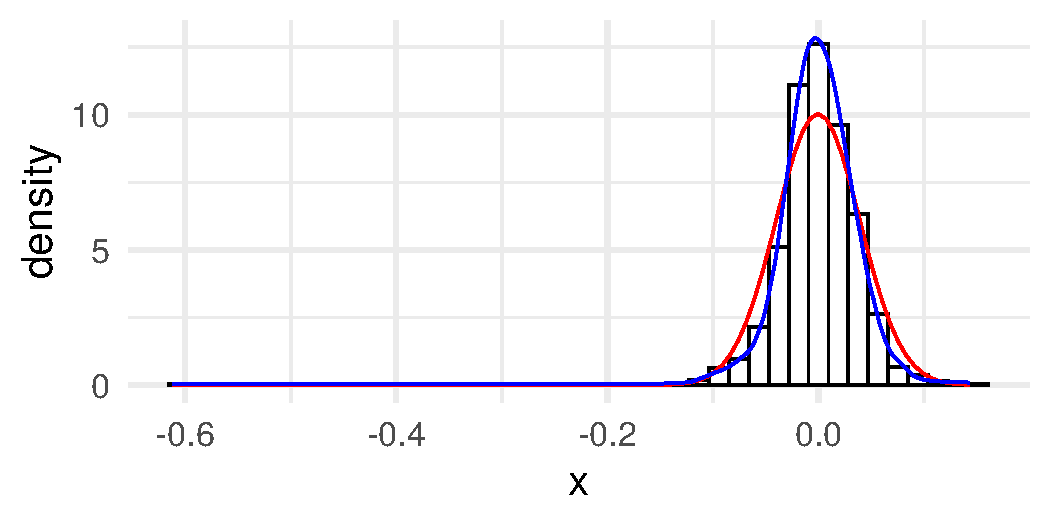
\includegraphics[width=\maxwidth]{figure/unnamed-chunk-33-1} 

\end{knitrout}


\begin{knitrout}
\definecolor{shadecolor}{rgb}{1, 1, 1}\color{fgcolor}\begin{kframe}
\begin{alltt}
\hlstd{fani} \hlkwb{<-} \hlkwd{tibble}\hlstd{()}

\hlkwa{for} \hlstd{(b} \hlkwa{in} \hlkwd{seq}\hlstd{(}\hlnum{0.001}\hlstd{,} \hlnum{0.05}\hlstd{,} \hlkwc{length.out} \hlstd{=} \hlnum{40}\hlstd{)) \{}
 \hlstd{f} \hlkwb{<-}
   \hlkwd{npudens}\hlstd{(}
     \hlkwc{tdat} \hlstd{= x,}
     \hlkwc{ckertype} \hlstd{=} \hlstr{"epanechnikov"}\hlstd{,}
     \hlkwc{bandwidth.compute} \hlstd{=} \hlnum{FALSE}\hlstd{,}
     \hlkwc{bws} \hlstd{= b}
   \hlstd{)}
 \hlstd{fani} \hlkwb{<-}
   \hlstd{fani} \hlopt \hlkwd{bind_rows}\hlstd{(}\hlkwd{tibble}\hlstd{(}
     \hlkwc{xreal} \hlstd{=} \hlkwd{sort}\hlstd{(x),}
     \hlkwc{x} \hlstd{= f}\hlopt{$}\hlstd{eval}\hlopt{$}\hlstd{x,}
     \hlkwc{y} \hlstd{= f}\hlopt{$}\hlstd{dens,}
     \hlkwc{bw} \hlstd{= b}
   \hlstd{))}
\hlstd{\}}

\hlkwd{ggplot}\hlstd{(}\hlkwc{data} \hlstd{= fani)} \hlopt{+}
 \hlkwd{geom_line}\hlstd{(}\hlkwd{aes}\hlstd{(x, y),} \hlkwc{color} \hlstd{=} \hlstr{"blue"}\hlstd{)} \hlopt{+}
 \hlkwd{labs}\hlstd{(}\hlkwc{title} \hlstd{=} \hlkwd{paste0}\hlstd{(}\hlstr{"Ancho de banda = \{closest_state\}"}\hlstd{))} \hlopt{+}
 \hlkwd{transition_states}\hlstd{(bw)} \hlopt{+}
 \hlkwd{view_follow}\hlstd{()} \hlopt{+}
 \hlkwd{theme_minimal}\hlstd{(}\hlkwc{base_size} \hlstd{=} \hlnum{20}\hlstd{)}

\hlkwd{anim_save}\hlstd{(}\hlstr{"manual_figure/bandwidth-animation-np.gif"}\hlstd{)}
\end{alltt}
\end{kframe}
\end{knitrout}

 \includemedia[
 label=bandwidth,
 width=0.6\linewidth,height=0.45\linewidth,
 addresource=manual_figure/bandwidth-animation-np.mp4,
 transparent,
 %transparent player background
 activate=pageopen,
 %show VPlayer's right-click menu
 flashvars={
 source=manual_figure/bandwidth-animation-np.mp4
 &loop=true
 % loop video
 }
 ]{}{VPlayer.swf}

 \begin{tarea}{}{}
 Implementar el intervalo confianza visto en clase para estimadores de densidades por núcleos y visualizarlo de en ggplot. 

 \textbf{Si se atreven: ¿Se podría hacer una versión animada de ese gráfico para visualizar el significado real de este el intervalo de confianza?}
 \end{tarea}


\include{cap-1-estimacion-densidades-no-parametricas.Rtex}


% !TeX spellcheck = es_ES



\begin{knitrout}
\definecolor{shadecolor}{rgb}{1, 1, 1}\color{fgcolor}\begin{kframe}
\begin{alltt}
\hlkwd{library}\hlstd{(knitr)}
\end{alltt}
\end{kframe}
\end{knitrout}





\chapter{Jacknife y Bootstrap}

Suponga que se quiere estimar un intervalo de confianza para la media
\(\mu\) desconocida de un conjunto de datos \(X_{1},\ldots, X_{n}\)
que tiene distribución  \(\mathcal{N}\left(\mu ,\sigma^{2}\right)\).

Primero se  conoce que

\begin{equation*}
\sqrt{n}\left( \hat{\mu} - \mu \right)
\xrightarrow{\mathcal{L}} \mathcal{N}\left(0,\sigma^{2}\right),
\end{equation*}

y esto nos permite escribir el intervalo de confianza como

\begin{equation*}
\left[ \hat{\mu} - \hat{\sigma}z_{1-\frac{\alpha}{2}} ,
\hat{\mu} + \hat{\sigma}z_{1-\frac{\alpha}{2}}\right]
\end{equation*}

donde \(z_{1-\frac{\alpha}{2}}\) es el cuantil \(1-\frac{\alpha}{2}\)
de una normal estándar.

La expresión anterior es posible ya que el supuesto es que la
distribución de \(\hat{\theta}\) es normal.

\begin{pregunta}{}{}
    ¿Qué pasaría si este supuesto es falso o al menos no conocemos la
    distribución de \(\hat{\theta}\)?

    ¿Cómo podemos encontrar ese intervalo de confianza?
\end{pregunta}

\begin{cuidado}{}{}
    Para una muestra fija, el estimador anterior  \(\hat{\mu}\)
    solamente un valor.  No se conoce la distribución de \(\hat{\mu}\). Lo
    único que se puede estimar son valores puntuales como la media,
    varianza, mediana, etc, pero no sabemos nada de su distribución.
\end{cuidado}

\subsection{Caso concreto}

Suponga que tenemos la siguiente tabla de datos, que representa una
muestra de tiempos y distancias de viajes en Atlanta.

Cargamos la base de la siguiente forma:

\begin{knitrout}
\definecolor{shadecolor}{rgb}{1, 1, 1}\color{fgcolor}\begin{kframe}
\begin{alltt}
\hlstd{CommuteAtlanta} \hlkwb{<-} \hlkwd{read.csv2}\hlstd{(}\hlstr{"data/CommuteAtlanta.csv"}\hlstd{)}
\hlkwd{kable}\hlstd{(}\hlkwd{head}\hlstd{(CommuteAtlanta))}
\end{alltt}
\end{kframe}
\begin{tabular}{l|r|r|r|l}
\hline
City & Age & Distance & Time & Sex\\
\hline
Atlanta & 19 & 10 & 15 & M\\
\hline
Atlanta & 55 & 45 & 60 & M\\
\hline
Atlanta & 48 & 12 & 45 & M\\
\hline
Atlanta & 45 & 4 & 10 & F\\
\hline
Atlanta & 48 & 15 & 30 & F\\
\hline
Atlanta & 43 & 33 & 60 & M\\
\hline
\end{tabular}


\end{knitrout}


Para este ejemplo tomaremos la variable \texttt{Time} que la
llamaremos \texttt{x} para ser más breves. En este caso note que

\begin{knitrout}
\definecolor{shadecolor}{rgb}{1, 1, 1}\color{fgcolor}\begin{kframe}
\begin{alltt}
\hlstd{x} \hlkwb{<-} \hlstd{CommuteAtlanta}\hlopt{$}\hlstd{Time}
\end{alltt}
\end{kframe}
\end{knitrout}


\begin{knitrout}
\definecolor{shadecolor}{rgb}{1, 1, 1}\color{fgcolor}\begin{kframe}
\begin{alltt}
\hlkwd{mean}\hlstd{(x)}
\end{alltt}
\begin{verbatim}
## [1] 29.11
\end{verbatim}
\end{kframe}
\end{knitrout}


y su varianza es

\begin{knitrout}
\definecolor{shadecolor}{rgb}{1, 1, 1}\color{fgcolor}\begin{kframe}
\begin{alltt}
\hlstd{(Tn} \hlkwb{<-} \hlkwd{var}\hlstd{(x))}
\end{alltt}
\begin{verbatim}
## [1] 429.2484
\end{verbatim}
\end{kframe}
\end{knitrout}


A partir de estos dos valores, ¿Cuál sería un intervalo de confianza
para la media?

Note que esta pregunta es difícil ya que no tenemos ningún tipo de
información adicional.

Las dos técnicas que veremos a continuación nos permitirán extraer
\emph{información adicional} de la muestra.

\begin{nota}{}{}
    Para efectos de este capítulo, llamaremos \(T_{n}=T\left(
    X_{1},\ldots,X_{n}\right)\) al estadístico formado por la muestra de
    los \(X_{i}\)'s.
\end{nota}

\newpage

\section{Jacknife}

Esta técnica fue propuesta por \cite{Quenouille1949} y consiste en la
siguiente observación.

Se puede probar que muchos de los estimadores tiene la propiedad que

\begin{equation}
\operatorname{Sesgo}\left(T_{n}\right)=\frac{a}{n}+\frac{b}{n^{2}}+O\left(\frac{1}{n^{3}}\right)
\end{equation}

para algún $a$ and $b$.

Por ejemplo $\sigma^{2}=\mathrm{Var}\left(X_{i}\right)$ y sea
$\widehat{\sigma}_{n}^{2}=n^{-1} \sum_{i=1}^{n}\left(X_{i}-\right.$
$\bar{X})^{2}$. Entonces,

\begin{equation*}
\mathbb{E}\left(\widehat{\sigma}_{n}^{2}\right)=
\frac{n-1}{n}\sigma^{2}
\end{equation*}

por lo tanto

\begin{equation*}
\mathrm{Sesgo} = -\frac{\sigma^{2}}{n}
\end{equation*}

Por lo tanto en este caso $a=-\sigma^{2}$ y $b=0$.

Defina \(T_{(-i)}\) como el estimador \(T_{n}\) pero eliminando el
\(i\)-ésimo término.

Es claro que en este contexto, se tiene que

\begin{equation}
\operatorname{Sesgo}\left(T_{(-i)}\right)=\frac{a}{n-1}+\frac{b}{(n-1)^{2}}+O\left(\frac{1}{(n-1)^{3}}\right)
\end{equation}

\begin{laboratorio}{}{}
    Una forma fácil de construir los \(T_{(-i)}\) es primero replicando
    la matriz de datos múltiple veces usando el producto de kronecker

\begin{knitrout}
\definecolor{shadecolor}{rgb}{1, 1, 1}\color{fgcolor}\begin{kframe}
\begin{alltt}
\hlstd{n} \hlkwb{<-} \hlkwd{length}\hlstd{(x)}
\hlstd{jackdf} \hlkwb{<-} \hlkwd{kronecker}\hlstd{(}\hlkwd{matrix}\hlstd{(}\hlnum{1}\hlstd{,} \hlnum{1}\hlstd{, n), x)}

\hlkwd{kable}\hlstd{(jackdf[}\hlnum{1}\hlopt{:}\hlnum{10}\hlstd{,} \hlnum{1}\hlopt{:}\hlnum{10}\hlstd{])}
\end{alltt}
\end{kframe}
\begin{tabular}{r|r|r|r|r|r|r|r|r|r}
\hline
15 & 15 & 15 & 15 & 15 & 15 & 15 & 15 & 15 & 15\\
\hline
60 & 60 & 60 & 60 & 60 & 60 & 60 & 60 & 60 & 60\\
\hline
45 & 45 & 45 & 45 & 45 & 45 & 45 & 45 & 45 & 45\\
\hline
10 & 10 & 10 & 10 & 10 & 10 & 10 & 10 & 10 & 10\\
\hline
30 & 30 & 30 & 30 & 30 & 30 & 30 & 30 & 30 & 30\\
\hline
60 & 60 & 60 & 60 & 60 & 60 & 60 & 60 & 60 & 60\\
\hline
45 & 45 & 45 & 45 & 45 & 45 & 45 & 45 & 45 & 45\\
\hline
10 & 10 & 10 & 10 & 10 & 10 & 10 & 10 & 10 & 10\\
\hline
25 & 25 & 25 & 25 & 25 & 25 & 25 & 25 & 25 & 25\\
\hline
15 & 15 & 15 & 15 & 15 & 15 & 15 & 15 & 15 & 15\\
\hline
\end{tabular}


\end{knitrout}


    Y luego se elimina la diagonal

\begin{knitrout}
\definecolor{shadecolor}{rgb}{1, 1, 1}\color{fgcolor}\begin{kframe}
\begin{alltt}
\hlkwd{diag}\hlstd{(jackdf)} \hlkwb{<-} \hlnum{NA}

\hlkwd{kable}\hlstd{(jackdf[}\hlnum{1}\hlopt{:}\hlnum{10}\hlstd{,} \hlnum{1}\hlopt{:}\hlnum{10}\hlstd{])}
\end{alltt}
\end{kframe}
\begin{tabular}{r|r|r|r|r|r|r|r|r|r}
\hline
NA & 15 & 15 & 15 & 15 & 15 & 15 & 15 & 15 & 15\\
\hline
60 & NA & 60 & 60 & 60 & 60 & 60 & 60 & 60 & 60\\
\hline
45 & 45 & NA & 45 & 45 & 45 & 45 & 45 & 45 & 45\\
\hline
10 & 10 & 10 & NA & 10 & 10 & 10 & 10 & 10 & 10\\
\hline
30 & 30 & 30 & 30 & NA & 30 & 30 & 30 & 30 & 30\\
\hline
60 & 60 & 60 & 60 & 60 & NA & 60 & 60 & 60 & 60\\
\hline
45 & 45 & 45 & 45 & 45 & 45 & NA & 45 & 45 & 45\\
\hline
10 & 10 & 10 & 10 & 10 & 10 & 10 & NA & 10 & 10\\
\hline
25 & 25 & 25 & 25 & 25 & 25 & 25 & 25 & NA & 25\\
\hline
15 & 15 & 15 & 15 & 15 & 15 & 15 & 15 & 15 & NA\\
\hline
\end{tabular}


\end{knitrout}


    Cada columna contiene toda la muestra excepto el \(i\)-ésimo
    elemento. Solo basta estimar la media de cada columna:

\begin{knitrout}
\definecolor{shadecolor}{rgb}{1, 1, 1}\color{fgcolor}\begin{kframe}
\begin{alltt}
\hlstd{T_i} \hlkwb{<-} \hlkwd{apply}\hlstd{(jackdf,} \hlnum{2}\hlstd{, var,} \hlkwc{na.rm}\hlstd{=}\hlnum{TRUE}\hlstd{)}

\hlkwd{kable}\hlstd{(T_i[}\hlnum{1}\hlopt{:}\hlnum{10}\hlstd{])}
\end{alltt}
\end{kframe}
\begin{tabular}{r}
\hline
x\\
\hline
429.7098\\
\hline
428.1905\\
\hline
429.6023\\
\hline
429.3756\\
\hline
430.1087\\
\hline
428.1905\\
\hline
429.6023\\
\hline
429.3756\\
\hline
430.0764\\
\hline
429.7098\\
\hline
\end{tabular}


\end{knitrout}


\end{laboratorio}

Definamos el sesgo \emph{jackife} como



\begin{equation*}
b_{jack} = (n-1) (\overline{T}_{n} - T_{n})
\end{equation*}

donde
\begin{equation*}
\overline{T}_{n} = \frac{1}{n} \sum_{i=1}^{n} T_{(-i)}
\end{equation*}


\begin{laboratorio}{}{}
    En nuestro caso tendríamos lo siguiente:

\begin{knitrout}
\definecolor{shadecolor}{rgb}{1, 1, 1}\color{fgcolor}\begin{kframe}
\begin{alltt}
\hlstd{(bjack} \hlkwb{<-} \hlstd{(n}\hlopt{-}\hlnum{1}\hlstd{)}\hlopt{*}\hlstd{(}\hlkwd{mean}\hlstd{(T_i)} \hlopt{-} \hlstd{Tn))}
\end{alltt}
\begin{verbatim}
## [1] 0
\end{verbatim}
\end{kframe}
\end{knitrout}


    es decir, que los \texttt{T\_i} generan estimadores de \texttt{T\_n}
    que contienen el mismo sesgo.
\end{laboratorio}

Observe que \(b_{jack}\) tiene la siguiente propiedad


\begin{align*}
\mathbb{E}\left(b_{\text {jack}}\right)
&= (n-1)\left(\mathbb{E}\left[\overline{T}_{n}\right] -
\mathbb{E}\left[T_{n}\right]\right) \\
&= (n-1)\left(\mathbb{E}\left[\overline{T}_{n}\right] - \theta +
\theta - \mathbb{E}\left[T_{n}\right]\right) \\
& =(n-1)\left(\mathrm{Sesgo} \left(\overline{T}_{n}\right)
-\mathrm{Sesgo}\left(T_{n}\right)\right) \\
& =(n-1)\left[\left(\frac{1}{n-1}
-\frac{1}{n}\right)
a+\left(\frac{1}{(n-1)^{2}}
-\frac{1}{n^{2}}\right) b+O\left(\frac{1}{n^{3}}\right)\right] \\
& =\frac{a}{n}
+\frac{(2 n-1) b}{n^{2}(n-1)}
+O\left(\frac{1}{n^{2}}\right) \\
& =\operatorname{Sesgo}\left(T_{n}\right)
+O\left(\frac{1}{n^{2}}\right)\\
\end{align*}

\begin{nota}{}{}
    Es decir, en general, el estimador \(b_{\text{jack}}\)  aproxima
    correctamente \(\mathrm{Sesgo}\left( T_{n} \right)\) hasta con un
    error del \(n^{-2}\).
\end{nota}


Podemos usar los \emph{T\_i} para generar muestras adicionales para
estimar el parámetro \(\theta\).

En este caso  defina el siguiente estimador:

\[
\widetilde{T}_{i}=n T_{n}-(n-1) T_{(-i)}.
\]

\begin{nota}{}{}
    A \(\widetilde{T}_{i}\) se le llaman \textbf{pseudo-valores} y
    representa el aporte o peso que tiene la variable \(X_{i}\) para
    estimar \(T_{n}\).
\end{nota}

\begin{tarea}{}{}
    Usado un cálculo similar para el \(b_{jack}\) pruebe que

    \[
    \operatorname{Sesgo}\left(T_{\text {jack}
    }\right)=-\frac{b}{n(n-1)}+O\left(\frac{1}{n^{2}}\right)=O\left(\frac{1}{n^{2}}\right).
    \]

    ¿Qué conclusión se obtiene de este cálculo?
\end{tarea}


\begin{laboratorio}{}{}
    Los pseudo-valores se estiman de forma directa como,

\begin{knitrout}
\definecolor{shadecolor}{rgb}{1, 1, 1}\color{fgcolor}\begin{kframe}
\begin{alltt}
\hlstd{pseudo} \hlkwb{<-} \hlstd{n} \hlopt{*} \hlstd{Tn} \hlopt{-} \hlstd{(n} \hlopt{-} \hlnum{1}\hlstd{)} \hlopt{*} \hlstd{T_i}

\hlstd{pseudo[}\hlnum{1}\hlopt{:}\hlnum{10}\hlstd{]}
\end{alltt}
\begin{verbatim}
##  [1] 199.02972209 957.16225222 252.64417993 365.79679037  -0.06666345
##  [6] 957.16225222 252.64417993 365.79679037  16.09799519 199.02972209
\end{verbatim}
\end{kframe}
\end{knitrout}



    Lo importante acá es notar la similitud que tiene con los datos
    reales,

\begin{knitrout}
\definecolor{shadecolor}{rgb}{1, 1, 1}\color{fgcolor}\begin{kframe}
\begin{alltt}
\hlkwd{plot}\hlstd{(}\hlkwc{x} \hlstd{= x,} \hlkwc{y} \hlstd{= pseudo)}
\end{alltt}
\end{kframe}
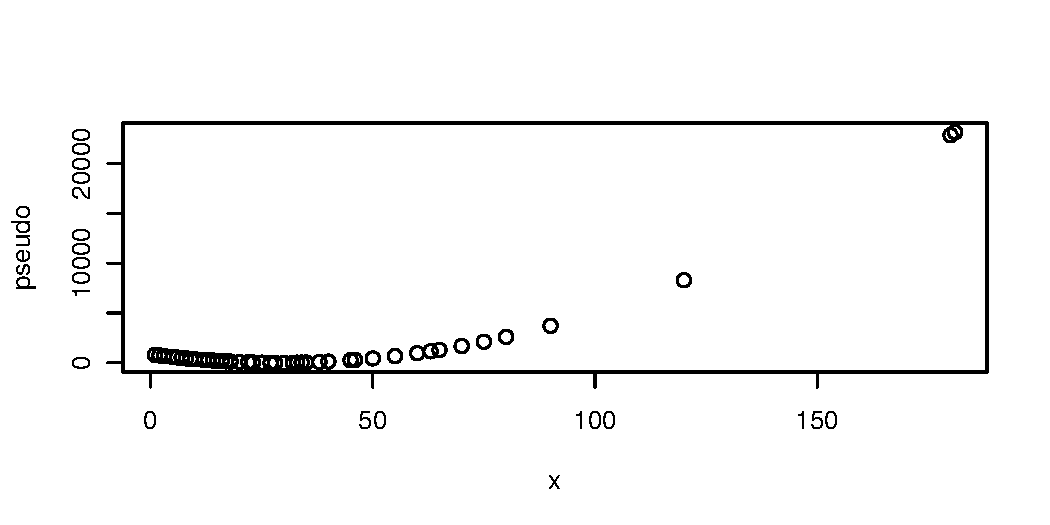
\includegraphics[width=\maxwidth]{figure/unnamed-chunk-40-1} 

\end{knitrout}


\end{laboratorio}

Con estos pseudo-valores, es posible estimar la media y la varianza de
\(T_{n}\) con sus respectivos estimadores:

\[
T_{\text {jack }}=\frac{1}{n} \sum_{i=1}^{n} \widetilde{T}_{i}
\]

donde

\[
v_{jack}=\frac{\sum_{i=1}^{n}\left(\widetilde{T}_{i}-\frac{1}{n}
    \sum_{i=1}^{n} \widetilde{T}_{i}\right)^{2}}{n(n-1)}.
\]



\begin{nota}{}{}

    Sin embargo, se puede demostrar fácilmente que se pueden usar
    pseudovalores para construir una prueba normal de hipótesis. Dado que
    cada pseudovalor es independiente e idénticamente distribuido (iid),
    se deduce que su promedio se ajusta a una distribución normal a medida
    que el tamaño de la muestra aumenta. El promedio de los pseudovalores
    es solo \(T_ {jack}\) y el valor esperado de ese promedio, debido a la
    construcción a la imparcialidad del estimador, es el parámetro bajo
    investigación, \(\theta \). Por lo tanto, tenemos que
    \[
    \frac{\sqrt{n}\left(T_{jack}-\theta\right)}{\sqrt{v_{jack}}}
    \rightarrow N(0,1).
    \]
\end{nota}


\begin{laboratorio}{}{}


\begin{knitrout}
\definecolor{shadecolor}{rgb}{1, 1, 1}\color{fgcolor}\begin{kframe}
\begin{alltt}
\hlstd{(Tjack} \hlkwb{<-} \hlkwd{mean}\hlstd{(pseudo))}
\end{alltt}
\begin{verbatim}
## [1] 429.2484
\end{verbatim}
\end{kframe}
\end{knitrout}



\begin{knitrout}
\definecolor{shadecolor}{rgb}{1, 1, 1}\color{fgcolor}\begin{kframe}
\begin{alltt}
\hlstd{(Vjack} \hlkwb{<-} \hlkwd{var}\hlstd{(pseudo,} \hlkwc{na.rm} \hlstd{=} \hlnum{TRUE}\hlstd{))}
\end{alltt}
\begin{verbatim}
## [1] 2701991
\end{verbatim}
\end{kframe}
\end{knitrout}



\begin{knitrout}
\definecolor{shadecolor}{rgb}{1, 1, 1}\color{fgcolor}\begin{kframe}
\begin{alltt}
\hlstd{(sdjack} \hlkwb{<-} \hlkwd{sqrt}\hlstd{(Vjack))}
\end{alltt}
\begin{verbatim}
## [1] 1643.774
\end{verbatim}
\end{kframe}
\end{knitrout}



\begin{knitrout}
\definecolor{shadecolor}{rgb}{1, 1, 1}\color{fgcolor}\begin{kframe}
\begin{alltt}
\hlstd{(z} \hlkwb{<-} \hlkwd{qnorm}\hlstd{(}\hlnum{1} \hlopt{-} \hlnum{0.05} \hlopt{/} \hlnum{2}\hlstd{))}
\end{alltt}
\begin{verbatim}
## [1] 1.959964
\end{verbatim}
\end{kframe}
\end{knitrout}



\begin{knitrout}
\definecolor{shadecolor}{rgb}{1, 1, 1}\color{fgcolor}\begin{kframe}
\begin{alltt}
\hlkwd{c}\hlstd{(Tjack} \hlopt{-} \hlstd{z} \hlopt{*} \hlstd{sdjack} \hlopt{/} \hlkwd{sqrt}\hlstd{(n),}
\hlstd{Tjack} \hlopt{+} \hlstd{z} \hlopt{*} \hlstd{sdjack} \hlopt{/} \hlkwd{sqrt}\hlstd{(n))}
\end{alltt}
\begin{verbatim}
## [1] 285.1679 573.3289
\end{verbatim}
\end{kframe}
\end{knitrout}




\end{laboratorio}


\newpage


\section{Bootstrap}


Este método es un poco más sencillo de implementar que Jacknife y es
igualmente de eficaz propuesto por \cite{Efron1979}.

Primero recordemos que estamos estimando una estadístico a partir de
una muestra de modo que \(T_{n}=g\left( X_{1},\ldots,X_{n} \right)\)
donde \(g\) es cualquier función (media, varianza, quantiles, etc).


Supongamos que conocemos la distribución real de los \(X\)'s, llamada \(F(x)\). Si uno
quisiera estimar la varianza de \(X\) basta con hacer

\begin{equation*}
\mathrm{Var}_{F}\left(T_{n}\right)
= \frac{\sigma^{2}}{n}=\frac{\int x^{2}  dF(x)-\left(\int x
dF(x)\right)^{2}}{n}
\end{equation*}



donde \(\sigma^{2} = \mathrm{Var}\left(X\right)\) y el subindice \(F\) es solo para indicar la dependencia con la distribución real.

Ahora dado que no tenemos la distribución  real \(F(x)\), una opción es encontrar un estimador de esta llamado \(\hat{F}_n\).

La técnica de boostrap se basa en extraer muchas muestras iid de la distribución \(\hat{F}_n\) de modo que se pueda conocer su varianza.

En simple pasos la técnica es

\begin{enumerate}
    \item Seleccione \(X_{1}^{*}, \ldots, X_{n}^{*} \sim \widehat{F}_{n}\)
    \item Estime \(T_{n}^{*}=g\left(X_{1}^{*}, \ldots, X_{n}^{*}\right)\)
    \item Repita los Pasos 1 y 2, \(B\) veces para obtener \(T_{n, 1}^{*}, \ldots, T_{n, B}^{*}\)
    \item Estime
    \[
    v_{\mathrm{boot}}=\frac{1}{B} \sum_{b=1}^{B}\left(T_{n, b}^{*}-\frac{1}{B} \sum_{r=1}^{B} T_{n, r}^{*}\right)^{2}
    \]
\end{enumerate}
Por la ley de los grandes números tenemos que

\begin{equation}
v_{\mathrm{boot}} \stackrel{\mathrm{a.s.}}{\longrightarrow} \mathbb{V}_{\widehat{F}_{n}}\left(T_{n}\right), \text {\quad si } B \rightarrow \infty.
\end{equation}

además llamaremos,

\begin{equation*}
\widehat{\mathrm{se}}_{\mathrm{boot}}=\sqrt{v_{\mathrm{boot}}}
\end{equation*}

En pocas palabras lo que tenemos es que


\begin{align*}
\text  {Mundo Real: }
& F
& \Longrightarrow  X_{1}, \ldots, X_{n}
& \Longrightarrow
& T_{n} = g\left(X_{1}, \ldots, X_{n}\right) \\
\text {Mundo Bootstrap: }
& \widehat{F}_{n}
& \Longrightarrow  X_{1}^{*}, \ldots, X_{n}^{*}
& \Longrightarrow
& T_{n}^{*}=g\left(X_{1}^{*}, \ldots, X_{n}^{*}\right)
\end{align*}

En términos de convergencia lo que se tiene es que
\[
\mathrm{Var}_{F}\left(T_{n}\right) \overbrace{\approx}^{O(1 / \sqrt{n})} \mathrm{Var}_{\widehat{F}_{n}}\left(T_{n}\right) \overbrace{\approx}^{O(1 / \sqrt{B})} v_{b o o t}
\]

\begin{pregunta}{}{}
    ¿Cómo extraemos una muestra de \(\hat{F}_n\)?
\end{pregunta}


Recuerden que \(\hat{F}_{n}\) asigna la probabilidad de \(\frac{1}{n}\) a cada valor usado para construirla.

Por lo tanto, todos los puntos originales \(X_{1},\ldots,X_{n}\) tienen probabilidad \(\frac{1}{n}\) de ser escogidos, que resulta ser equivalente a un muestreo con remplazo \(n\)-veces.

 Así que basta cambiar el punto 1. del algoritmo mencionando anteriormente con

\begin{enumerate}
        \item Seleccione una muestra con remplazo  \(X_{1}^{*}, \ldots, X_{n}^{*}\) de  \(X_{1},\ldots,X_{n}\).
\end{enumerate}

\begin{laboratorio}{}{}
   En este ejemplo podemos tomar \(B=1000\) y construir esa cantidad de veces nuestro estimador.

\begin{knitrout}
\definecolor{shadecolor}{rgb}{1, 1, 1}\color{fgcolor}\begin{kframe}
\begin{alltt}
\hlstd{B} \hlkwb{<-} \hlnum{1000}
\hlstd{Tboot_b} \hlkwb{<-} \hlkwa{NULL}

\hlkwa{for}\hlstd{(b} \hlkwa{in} \hlnum{1}\hlopt{:}\hlstd{B) \{}
\hlstd{xb} \hlkwb{<-} \hlkwd{sample}\hlstd{(x,} \hlkwc{size} \hlstd{= n,} \hlkwc{replace} \hlstd{=} \hlnum{TRUE}\hlstd{)}
\hlstd{Tboot_b[b]} \hlkwb{<-} \hlkwd{var}\hlstd{(xb)}
\hlstd{\}}


\hlstd{Tboot_b[}\hlnum{1}\hlopt{:}\hlnum{10}\hlstd{]}
\end{alltt}
\begin{verbatim}
##  [1] 384.8959 439.3992 540.4429 356.0363 382.5001 539.7398 389.2075 355.4033
##  [9] 371.0053 469.0120
\end{verbatim}
\end{kframe}
\end{knitrout}


\begin{knitrout}
\definecolor{shadecolor}{rgb}{1, 1, 1}\color{fgcolor}\begin{kframe}
\begin{alltt}
\hlkwd{plot}\hlstd{(Tboot_b)}
\end{alltt}
\end{kframe}
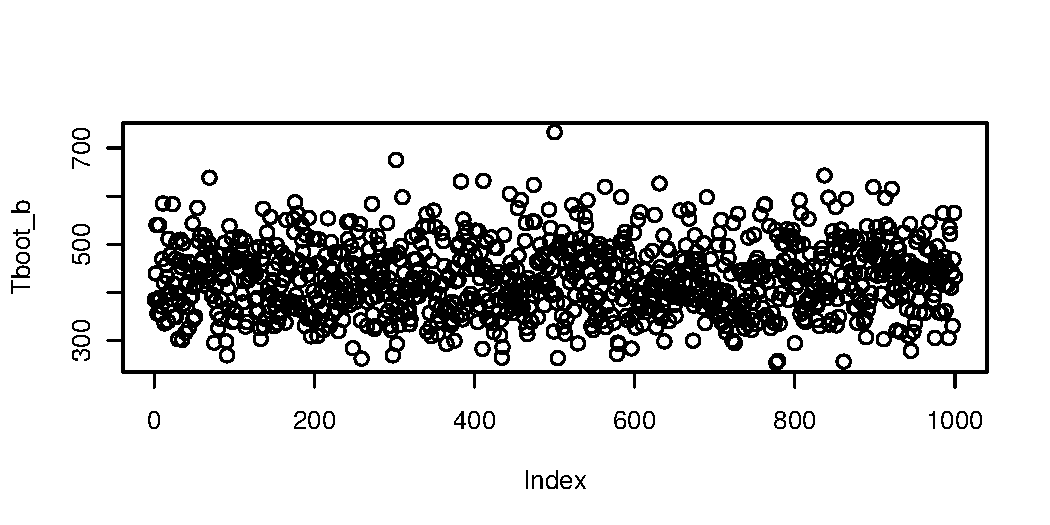
\includegraphics[width=\maxwidth]{figure/unnamed-chunk-47-1} 

\end{knitrout}


   Por supuesto podemos encontrar los estadísticos usuales para esta nueva muestra

\begin{knitrout}
\definecolor{shadecolor}{rgb}{1, 1, 1}\color{fgcolor}\begin{kframe}
\begin{alltt}
\hlstd{(Tboot} \hlkwb{<-} \hlkwd{mean}\hlstd{(Tboot_b))}
\end{alltt}
\begin{verbatim}
## [1] 428.3197
\end{verbatim}
\end{kframe}
\end{knitrout}


\begin{knitrout}
\definecolor{shadecolor}{rgb}{1, 1, 1}\color{fgcolor}\begin{kframe}
\begin{alltt}
\hlstd{(Vboot} \hlkwb{<-} \hlkwd{var}\hlstd{(Tboot_b))}
\end{alltt}
\begin{verbatim}
## [1] 5345.401
\end{verbatim}
\end{kframe}
\end{knitrout}


\begin{knitrout}
\definecolor{shadecolor}{rgb}{1, 1, 1}\color{fgcolor}\begin{kframe}
\begin{alltt}
\hlstd{(sdboot} \hlkwb{<-} \hlkwd{sqrt}\hlstd{(Vboot))}
\end{alltt}
\begin{verbatim}
## [1] 73.11225
\end{verbatim}
\end{kframe}
\end{knitrout}

\end{laboratorio}

\subsection{Intervalos de confianza}



\subsubsection{Intervalo Normal}

Este es el más sencillo y se escribe como

\begin{equation}
T_{n} \pm z_{\alpha / 2} \widehat{\mathrm{Se}}_{\mathrm{boot}}
\end{equation}

\begin{cuidado}{}{}
    Este intervalo solo funciona si la distribución de \(T_{n}\) es normal.
\end{cuidado}

\begin{laboratorio}{}{}
    El cálculo de este intervalo es
\begin{knitrout}
\definecolor{shadecolor}{rgb}{1, 1, 1}\color{fgcolor}\begin{kframe}
\begin{alltt}
\hlkwd{c}\hlstd{(Tn} \hlopt{-} \hlstd{z} \hlopt{*} \hlstd{sdboot,}
\hlstd{Tn} \hlopt{+} \hlstd{z} \hlopt{*} \hlstd{sdboot)}
\end{alltt}
\begin{verbatim}
## [1] 285.9510 572.5458
\end{verbatim}
\end{kframe}
\end{knitrout}

\end{laboratorio}

\subsubsection{Intervalo pivotal}

Sea  \(\theta=T(F)\) y  \(\widehat{\theta}_{n}=T\left(\widehat{F}_{n}\right)\) y defina la cantidad pivotal  \(R_{n}=\widehat{\theta}_{n}-\theta .\)

Sea  \(H(r)\) la función de distribución del pivote:
\[
H(r)=\mathbb{P}_{F}\left(R_{n} \leq r\right).
\]

Además considere  \(C_{n}^{\star}=(a, b)\)  donde
\[
a=\widehat{\theta}_{n}-H^{-1}\left(1-\frac{\alpha}{2}\right) \quad \text { y } \quad b=\widehat{\theta}_{n}-H^{-1}\left(\frac{\alpha}{2}\right).
\]

Se sigue que
\begin{align*}
\mathbb{P}(a \leq \theta \leq b)
&=\mathbb{P}\left(\widehat{\theta}_{n}-b \leq R_{n} \leq \widehat{\theta}_{n}-a\right) \\
&=H\left(\widehat{\theta}_{n}-a\right)-H\left(\widehat{\theta}_{n}-b\right) \\
&=H\left(H^{-1}\left(1-\frac{\alpha}{2}\right)\right)-H\left(H^{-1}\left(\frac{\alpha}{2}\right)\right) \\
&=1-\frac{\alpha}{2}-\frac{\alpha}{2}=1-\alpha
\end{align*}
\begin{nota}{}{}
     \(C_{n}^{\star}=(a, b)\)  es un intervalo de confianza al \(1-\alpha\) de confianza.

     El problema es que este intervalo depende de \(H\) desconocido.

\end{nota}


Para resolver este problema, se puede construir una versión \emph{bootstrap} de \(H\) usando lo que sabemos hasta ahora.

\[
\widehat{H}(r)=\frac{1}{B} \sum_{b=1}^{B} I\left(R_{n, b}^{*} \leq r\right)
\]
donde \(R_{n, b}^{*}=\widehat{\theta}_{n, b}^{*}-\widehat{\theta}_{n}\).

Sea  \(r_{\beta}^{*}\) el cuantil muestral de tamaño  \(\beta\) de  \(\left(R_{n, 1}^{*}, \ldots, R_{n, B}^{*}\right)\) y sea \(\theta_{\beta}^{*}\) el cuantil muestral de tamaño  \(\beta\) de \(\left(\theta_{n, 1}^{*}, \ldots, \theta_{n, B}^{*}\right)\).
\begin{nota}{}{}
    Según la notación anterior note que
    \begin{equation*}
    r_{\beta}^{*}= \theta_{\beta}^{*}-\widehat{\theta}_{n}
    \end{equation*}
\end{nota}



 Con estas observaciones
  It follows that an approximate \(1-\alpha\) confidence interval is \(C_{n}=(\widehat{a}, \widehat{b})\) where

\begin{align*}
\widehat{a}
&= \widehat{\theta}_{n}-\widehat{H}^{-1}\left(1-\frac{\alpha}{2}\right)
&= \widehat{\theta}_{n}-r_{1-\alpha / 2}^{*}
&= \widehat{\theta}_{n}-\theta_{1-\alpha / 2}^{*} + \widehat{\theta}_{n}
&=2 \widehat{\theta}_{n}-\theta_{1-\alpha / 2}^{*} \\
\widehat{b} &=\widehat{\theta}_{n}-\widehat{H}^{-1}\left(\frac{\alpha}{2}\right)
&=\widehat{\theta}_{n}-r_{\alpha / 2}^{*}
&= \widehat{\theta}_{n}-\theta_{\alpha / 2}^{*} + \widehat{\theta}_{n}
&=2 \widehat{\theta}_{n}-\theta_{\alpha / 2}^{*}
\end{align*}

\begin{nota}{}{}
    El intervalo de confianza pivotal de tamaño \(1-\alpha\) es
    \[
    C_{n}=\left(2 \widehat{\theta}_{n}-\widehat{\theta}_{((1-\alpha / 2) B)}^{*}, 2 \widehat{\theta}_{n}-\widehat{\theta}_{((\alpha / 2) B)}^{*}\right)
    \]
\end{nota}
\begin{laboratorio}{}{}
    El intervalo anterior para un nivel de 95\% se estima de la siguiente forma
\begin{knitrout}
\definecolor{shadecolor}{rgb}{1, 1, 1}\color{fgcolor}\begin{kframe}
\begin{alltt}
\hlkwd{c}\hlstd{(}\hlnum{2} \hlopt{*} \hlstd{Tn} \hlopt{-} \hlkwd{quantile}\hlstd{(Tboot_b,} \hlnum{1} \hlopt{-} \hlnum{0.05} \hlopt{/} \hlnum{2}\hlstd{) ,}
\hlnum{2} \hlopt{*} \hlstd{Tn} \hlopt{-} \hlkwd{quantile}\hlstd{(Tboot_b,} \hlnum{0.05} \hlopt{/} \hlnum{2}\hlstd{))}
\end{alltt}
\begin{verbatim}
##    97.5%     2.5% 
## 275.3768 558.6741
\end{verbatim}
\end{kframe}
\end{knitrout}

\end{laboratorio}

\subsubsection{Intervalo pivotal studentizado}

Una mejora del intervalo anterior sería normalizar los estimadores previamente

\[
Z_{n}=\frac{T_{n}-\theta}{\widehat{\mathrm{se}}_{\mathrm{boot}}}.
\]
Como \(\theta\) es desconocido, entonces la versión a estimar es
\[
Z_{n, b}^{*}=\frac{T_{n, b}^{*}-T_{n}}{\widehat{\mathrm{se}}_{b}^{*}}
\]
donde  \(\widehat{\mathrm{se}}_{b}^{*}\) es un estimador del error estándar de  \(T_{n, b}^{*}\) no de \(T_{n}\).

\begin{cuidado}{}{}
    Esto requerira estimar la varianza de \(T_{n,b}^*\) para cada \(b\).
\end{cuidado}

Con esto se puede obtener  cantidades \(Z_{n, 1}^{*}, \ldots, Z_{n, B}^{*}\) que debería ser próximos a \(Z_{n}\).

Sea \(z_{\alpha}^{*}\) del \(\alpha\) cuantiĺ de \(Z_{n, 1}^{*}, \ldots, Z_{n, B}^{*},\) entonces  \(\mathbb{P}\left(Z_{n} \leq z_{\alpha}^{*}\right) \approx \alpha\).

Define el intervalo
\begin{equation*}
C_{n}=\left(T_{n}-z_{1-\alpha / 2}^{*} \widehat{\mathrm{se}}_{\mathrm{boot}}, T_{n}-z_{\alpha / 2}^{*} \widehat{\mathrm{se}}_{\mathrm{boot}}\right)
\end{equation*}

Justificado por el siguiente cálculo:


\begin{align*}
\mathbb{P}\left(\theta \in C_{n}\right) &=\mathbb{P}\left(T_{n}-z_{1-\alpha / 2}^{*} \widehat{\mathrm{Se}}_{\mathrm{boot}} \leq \theta \leq T_{n}-z_{\alpha / 2}^{*} \widehat{\mathrm{Se}}_{\mathrm{boot}}\right) \\
&=\mathbb{P}\left(z_{\alpha / 2}^{*} \leq \frac{T_{n}-\theta}{\mathrm{se}_{\mathrm{boot}}} \leq z_{1-\alpha / 2}^{*}\right) \\
&=\mathbb{P}\left(z_{\alpha / 2}^{*} \leq Z_{n} \leq z_{1-\alpha / 2}^{*}\right) \\
& \approx 1-\alpha
\end{align*}

\begin{laboratorio}{}{}

    Note que para este caso tenemos que hacer bootstrap para cada estimador bootstrap calculado.
\begin{knitrout}
\definecolor{shadecolor}{rgb}{1, 1, 1}\color{fgcolor}\begin{kframe}
\begin{alltt}
   \hlstd{B} \hlkwb{<-} \hlnum{1000}
   \hlstd{Tboot_b} \hlkwb{<-} \hlkwa{NULL}
   \hlstd{Tboot_bm} \hlkwb{<-} \hlkwa{NULL}
   \hlstd{sdboot_b} \hlkwb{<-} \hlkwa{NULL}

   \hlkwa{for} \hlstd{(b} \hlkwa{in} \hlnum{1}\hlopt{:}\hlstd{B) \{}
 \hlstd{xb} \hlkwb{<-} \hlkwd{sample}\hlstd{(x,} \hlkwc{size} \hlstd{= n,} \hlkwc{replace} \hlstd{=} \hlnum{TRUE}\hlstd{)}
 \hlstd{Tboot_b[b]} \hlkwb{<-} \hlkwd{var}\hlstd{(xb)}
 \hlkwa{for} \hlstd{(m} \hlkwa{in} \hlnum{1}\hlopt{:}\hlstd{B) \{}
   \hlstd{xbm} \hlkwb{<-} \hlkwd{sample}\hlstd{(xb,} \hlkwc{size} \hlstd{= n,} \hlkwc{replace} \hlstd{=} \hlnum{TRUE}\hlstd{)}
   \hlstd{Tboot_bm[b]} \hlkwb{<-} \hlkwd{var}\hlstd{(xbm)}
 \hlstd{\}}
 \hlstd{sdboot_b} \hlkwb{<-} \hlkwd{sd}\hlstd{(Tboot_bm)}
   \hlstd{\}}

   \hlstd{z_star} \hlkwb{<-} \hlstd{(Tboot_b} \hlopt{-} \hlstd{Tn)} \hlopt{/} \hlstd{sdboot_b}

   \hlkwd{hist}\hlstd{(z_star)}
\end{alltt}
\end{kframe}
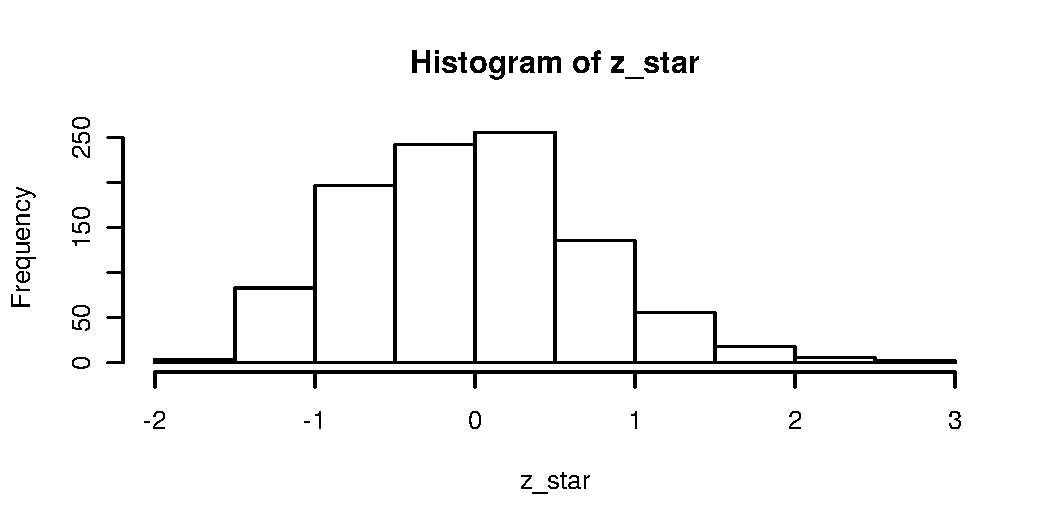
\includegraphics[width=\maxwidth]{figure/unnamed-chunk-53-1} 

\end{knitrout}


\begin{knitrout}
\definecolor{shadecolor}{rgb}{1, 1, 1}\color{fgcolor}\begin{kframe}
\begin{alltt}
\hlkwd{c}\hlstd{(Tn} \hlopt{-} \hlkwd{quantile}\hlstd{(z_star,} \hlnum{1} \hlopt{-} \hlnum{0.05} \hlopt{/} \hlnum{2}\hlstd{)} \hlopt{*}   \hlstd{sdboot,}
\hlstd{Tn} \hlopt{-} \hlkwd{quantile}\hlstd{(z_star,} \hlnum{0.05} \hlopt{/} \hlnum{2}\hlstd{)} \hlopt{*}   \hlstd{sdboot)}
\end{alltt}
\begin{verbatim}
##    97.5%     2.5% 
## 317.0387 519.9397
\end{verbatim}
\end{kframe}
\end{knitrout}

\end{laboratorio}


\subsection{Resumiendo}


Resumiendo todos lo métodos de cálculo de intervalos obtenemos

\begin{knitrout}
\definecolor{shadecolor}{rgb}{1, 1, 1}\color{fgcolor}\begin{kframe}
\begin{alltt}
   \hlkwd{kable}\hlstd{(}\hlkwd{data.frame}\hlstd{(}
     \hlkwc{`Método`} \hlstd{=} \hlkwd{c}\hlstd{(}
       \hlstr{"Jacknife"}\hlstd{,}
       \hlstr{"Bootstrap Normal"}\hlstd{,}
       \hlstr{"Bootstrap Pivotal"}\hlstd{,}
       \hlstr{"Bootstrap Pivotal Estudentizado"}
     \hlstd{),}
     \hlkwc{Inferior} \hlstd{=} \hlkwd{c}\hlstd{(}
       \hlstd{Tjack} \hlopt{-} \hlstd{z} \hlopt{*} \hlstd{sdjack} \hlopt{/} \hlkwd{sqrt}\hlstd{(n),}
       \hlstd{Tn} \hlopt{-} \hlstd{z} \hlopt{*} \hlstd{sdboot,}
       \hlnum{2} \hlopt{*} \hlstd{Tn} \hlopt{-} \hlkwd{quantile}\hlstd{(Tboot_b,} \hlnum{1} \hlopt{-} \hlnum{0.05} \hlopt{/} \hlnum{2}\hlstd{),}
       \hlstd{Tn} \hlopt{-} \hlkwd{quantile}\hlstd{(z_star,} \hlnum{1} \hlopt{-} \hlnum{0.05} \hlopt{/} \hlnum{2}\hlstd{)} \hlopt{*}   \hlstd{sdboot}
     \hlstd{),}
     \hlkwc{Superior} \hlstd{=} \hlkwd{c}\hlstd{(}
        \hlstd{Tjack} \hlopt{+} \hlstd{z} \hlopt{*} \hlstd{sdjack} \hlopt{/} \hlkwd{sqrt}\hlstd{(n),}
        \hlstd{Tn} \hlopt{+} \hlstd{z} \hlopt{*} \hlstd{sdboot,}
         \hlnum{2} \hlopt{*} \hlstd{Tn} \hlopt{-} \hlkwd{quantile}\hlstd{(Tboot_b,} \hlnum{0.05} \hlopt{/} \hlnum{2}\hlstd{),}
        \hlstd{Tn} \hlopt{-} \hlkwd{quantile}\hlstd{(z_star,} \hlnum{0.05} \hlopt{/} \hlnum{2}\hlstd{)} \hlopt{*}   \hlstd{sdboot}
     \hlstd{)}
   \hlstd{))}
\end{alltt}
\end{kframe}
\begin{tabular}{l|r|r}
\hline
Método & Inferior & Superior\\
\hline
Jacknife & 285.1679 & 573.3289\\
\hline
Bootstrap Normal & 285.9510 & 572.5458\\
\hline
Bootstrap Pivotal & 273.7930 & 554.8922\\
\hline
Bootstrap Pivotal Estudentizado & 317.0387 & 519.9397\\
\hline
\end{tabular}


\end{knitrout}


\section{Ejercicios}

\begin{enumerate}
    \item Repita los ejercicios anteriores para calcular intervalos de confianza para la distancia promedio y la varianza del desplazamiento de las personas. Use los métodos de Jacknife y Bootstrap (con todos sus intervalos de confianza).

    Dada que la distancia es una medida que puede ser influenciada por distancias muy cortas o muy largas, se puede calcular el logaritmo de esta variable para eliminar la escala de la distancias.

    \item Verifique que esta última variable se podría estimar paramétricamente con una distribución normal.

    Repita los cálculos anteriores tomando como cuantiles los de una normal con media 0 y varianza 1.

    \item Compare los intervalos calculados y comente los resultados.

\end{enumerate}

\include{cap-2-jacknife-bootstrap.Rtex}

\newpage
\printbibliography
\end{document}
